\documentclass[11pt]{article}
\usepackage[margin=0.82in]{geometry}
\usepackage{amsmath,amssymb,booktabs,graphicx,float,longtable,microtype,tabularx,xcolor}
\usepackage[colorlinks=true,linkcolor=blue!45!black,urlcolor=blue!45!black,citecolor=blue!45!black]{hyperref}
\hypersetup{
  pdftitle={Generative Modeling: Variational Autoencoders, Flows, and Diffusion},
  pdfauthor={MATH 550 Capstone Course Development},
  pdfsubject={Three-week graduate module with reproducible public-data validation}
}
\graphicspath{{../../output/generative/figures/}}
\definecolor{navy}{HTML}{1F4E78}
\definecolor{lightblue}{HTML}{D9EAF7}
\definecolor{warm}{HTML}{F5E7D3}
\setlength{\parindent}{0pt}
\setlength{\parskip}{4pt}
\newcommand{\code}[1]{\texttt{#1}}
\newcommand{\E}{\mathbb{E}}

\begin{document}

\begin{center}
{\LARGE\bfseries\color{navy} Generative Modeling}\\[4pt]
{\Large Variational Autoencoders, Flows, and Diffusion}\\[9pt]
{\large Detailed standalone lecture notes with reproducible evidence}\\[10pt]
MATH 550 Mathematical Data Science Capstone\\
\end{center}

\colorbox{lightblue}{\parbox{0.96\linewidth}{
\textbf{Executive finding.} The module makes three generative contracts
executable: a VAE optimizes a variational bound and decodes in one pass; flow
matching learns continuous transport; diffusion learns to reverse corruption. On the
public digits benchmark, the lowest mean latent-space Fr\'echet distance was
Gaussian mixture (classical baseline,
0.090). The flow-matching MLP-minus-linear
gap was +0.038; the diffusion capacity gap was
+0.021.
These are compact CPU demonstrations, not image-generation leaderboard claims.
The strongest caveat is the eight-dimensional PCA bottleneck, which retains
67.4\% of training-set variance and visibly limits sample sharpness.
Two-moons and original 28-by-28 MNIST demonstrations compare VAE and flow behavior
on the same data, while the lower-resolution benchmark supplies paired metrics.
}}

\section*{1. Communication job and learning outcomes}

This module is designed for graduate data-science, AI, and machine-learning
capstone students who already know multivariable calculus, probability,
linear algebra, and basic neural-network training. It is not an LLM unit.
After nine 60-minute units, students should be able to:

\begin{enumerate}
\item distinguish explicit-likelihood, latent-variable, adversarial, score-based,
and transport-based generators by objective, inference, and sampling cost;
\item derive the change-of-variables, ELBO, adversarial, denoising, and conditional
flow-matching objectives and state what each objective does \emph{not} guarantee;
\item construct a conditional probability path and its sample-wise velocity target;
\item define PyTorch encoder/decoder and time-conditioned modules, train them with
autograd and \code{torch.optim}, and run one-pass, ODE, or deterministic diffusion samplers;
\item diagnose fidelity, coverage, memorization risk, numerical error, and metric
misuse using multiple forms of evidence; and
\item justify a generative-model family for a capstone application under data,
compute, evaluation, uncertainty, and governance constraints.
\end{enumerate}

\section*{2. Three-week teaching sequence (nine units)}

\begin{longtable}{@{}p{0.08\linewidth}p{0.25\linewidth}p{0.42\linewidth}p{0.179\linewidth}@{}}
\toprule
Unit & Central question & Concepts and in-class work & Evidence of learning \\
\midrule
\endhead
1 & What does it mean to learn a distribution? & Pushforwards, density models,
implicit models, likelihood, sampling, conditioning; fidelity versus coverage;
why visual inspection is insufficient. & Metric critique and failure-mode sort. \\
2 & What is gained and lost by latent variables? & Autoregressive factorization,
VAE ELBO and reparameterization, amortized inference, posterior collapse; short
comparison with energy-based models. & ELBO derivation and model-selection memo. \\
3 & Why can adversarial training look good but fail silently? & GAN minimax game,
non-saturating loss, discriminator as density-ratio signal, instability, mode
collapse, evaluation and governance. & Two-distribution game exercise. \\
\midrule
4 & How can an invertible map model density exactly? & Change of variables,
Jacobian determinants, coupling layers, Real NVP, exact inverse and likelihood. &
Affine-coupling round-trip test. \\
5 & What changes in continuous time? & Neural ODEs, continuous normalizing flows,
continuity equation, instantaneous change of variables, Euler and RK4 error. &
ODE solver convergence lab. \\
6 & How does flow matching remove simulation from training? & Probability paths,
conditional paths, marginalization, independent coupling, OT coupling, velocity
regression, guidance and conditioning. & Implement conditional FM targets. \\
\midrule
7 & How does diffusion learn to reverse noise? & Forward Gaussian chain, schedules,
$\epsilon$/$x_0$/velocity parameterizations, denoising loss, ancestral sampling,
DDIM. & Derive forward marginal and code noise targets. \\
8 & Are diffusion and flow matching different languages for the same object? &
Scores, reverse-time SDE, probability-flow ODE, stochastic versus deterministic
samplers, path geometry, network evaluations. & Map formulas and compare samplers. \\
9 & What evidence justifies deployment? & Paired benchmark, sample quality and
coverage, memorization, conditional evaluation, reproducibility, data rights,
failure reporting, capstone design review. & Reproducible audit and decision memo. \\
\bottomrule
\end{longtable}

\textbf{Suggested weekly rhythm.} Each week uses roughly 100 minutes of
derivation, 55 minutes of live code/diagnostics, and 25 minutes of critique or
design work. The slide deck supplies three visible weekly sections; the report is
the technical record; the homework transfers the method to Fashion-MNIST.

\section*{3. A compact map of generative-model families}

\begin{table}[H]
\centering
\small
\begin{tabularx}{\linewidth}{p{0.14\linewidth}p{0.22\linewidth}p{0.18\linewidth}p{0.18\linewidth}X}
\toprule
Family & Training signal & Density & Sampling & Main teaching value / failure mode \\
\midrule
Autoregressive & exact next-element log likelihood & exact & sequential & exposes
factorization choices; slow sampling and order dependence \\
VAE & ELBO with amortized posterior & lower bound & one decoder pass & clean latent
inference; variational gap and posterior collapse \\
GAN & discriminator--generator game & implicit & one generator pass & direct sample
quality; unstable game and mode dropping \\
Normalizing flow & exact change-of-variables likelihood & exact & invertible pass &
auditable density/inverse; architectural Jacobian constraints \\
Diffusion / score & denoising or score regression & variational / ODE options &
iterative SDE/ODE & stable corruption task; many network evaluations \\
Flow matching & conditional velocity regression & CNF likelihood available & ODE &
simulation-free training and flexible paths; solver/path error still matters \\
Energy-based & unnormalized energy / score & partition function difficult & MCMC &
general compatibility modeling; expensive mixing and normalization \\
\bottomrule
\end{tabularx}
\caption{No family dominates every axis. ``Popular'' is not a sufficient selection criterion.}
\end{table}

\subsection*{3.1 Objectives students should be able to derive}

For an invertible map $x=f_\theta(z)$ with base density $p_Z$,
\[
 \log p_X(x)=\log p_Z(f_\theta^{-1}(x))
 +\log\left|\det J_{f_\theta^{-1}}(x)\right|.
\]
The VAE evidence lower bound is
\[
 \log p_\theta(x)\geq
 \E_{q_\phi(z\mid x)}[\log p_\theta(x\mid z)]
 -D_{\mathrm{KL}}(q_\phi(z\mid x)\Vert p(z)).
\]
The original GAN game is
\[
 \min_G\max_D\;\E_{x\sim p_{\rm data}}\log D(x)
 +\E_{z\sim p(z)}\log(1-D(G(z))).
\]
These objectives optimize different surrogates. Likelihood, perceptual fidelity,
coverage, and usefulness downstream are related but not interchangeable.

\subsection*{3.2 VAE derivation: bound, Gaussian KL, and pathwise gradients}

Introduce any normalized encoder $q_\phi(z\mid x)$ into the marginal likelihood:
\begin{align*}
\log p_\theta(x)
&=\log\int q_\phi(z\mid x)
\frac{p_\theta(x,z)}{q_\phi(z\mid x)}\,dz\\
&\geq \E_{q_\phi(z\mid x)}
\left[\log p_\theta(x,z)-\log q_\phi(z\mid x)\right]\\
&=\E_q[\log p_\theta(x\mid z)]
-D_{\mathrm{KL}}(q_\phi(z\mid x)\Vert p(z))
=:\mathcal L_{\rm ELBO}(x).
\end{align*}
The inequality is Jensen's inequality. Adding and subtracting the exact posterior
gives the identity
\[
\log p_\theta(x)=\mathcal L_{\rm ELBO}(x)
+D_{\mathrm{KL}}(q_\phi(z\mid x)\Vert p_\theta(z\mid x)).
\]
The nonnegative second term is the variational gap. An apparently well-optimized
bound can therefore remain loose because of the chosen approximate posterior.

For a diagonal Gaussian encoder and standard-normal prior,
\[
q_\phi(z\mid x)=\mathcal N\!\left(
\mu_\phi(x),\operatorname{diag}\sigma_\phi^2(x)\right),
\qquad p(z)=\mathcal N(0,I),
\]
the regularizer is analytic:
\[
D_{\mathrm{KL}}(q_\phi\Vert p)
=\frac12\sum_{j=1}^{d_z}
\left(\mu_j^2+\exp(\log\sigma_j^2)-1-\log\sigma_j^2\right).
\]
Direct sampling from a parameterized distribution blocks ordinary backpropagation
through the random draw. The reparameterization
\[
\epsilon\sim\mathcal N(0,I),\qquad
z=\mu_\phi(x)+\exp\!\left(\tfrac12\log\sigma_\phi^2(x)\right)
\odot\epsilon
\]
moves randomness into the parameter-free $\epsilon$. Conditioned on $\epsilon$,
$z$ is differentiable with respect to both posterior heads, so PyTorch autograd
produces a pathwise gradient estimator.

The implementation minimizes one Monte Carlo estimate of the negative ELBO:
\[
\widehat{\mathcal J}(x)
=-\log p_\theta(x\mid z)
+\beta D_{\mathrm{KL}}(q_\phi(z\mid x)\Vert p(z)),
\qquad \beta=1.
\]
For two moons and whitened PCA coordinates, $p_\theta(x\mid z)$ is an isotropic
Gaussian with declared fixed variance. Its reconstruction term is a scaled sum
of squared errors, up to a constant. For MNIST, the decoder uses independent
Bernoulli pixels, giving binary cross-entropy summed over 784 pixels. A mean over
pixels combined with a sum over latent dimensions would silently change the
effective $\beta$, so reductions are part of the mathematical specification.

\textbf{Two diagnostic paths must stay separate.} A reconstruction computes
$x\to q_\phi(z\mid x)\to p_\theta(x\mid z)$ and tests information preservation.
A new sample computes $z\sim p(z)\to p_\theta(x\mid z)$ and tests whether the
regularized aggregate posterior is compatible with the prior. Excellent
reconstruction can coexist with poor prior samples; the two-moons experiment
below demonstrates exactly that failure.

\section*{4. From normalizing flows to flow matching}

\subsection*{4.1 Continuous transport}

A time-dependent velocity $u_t$ defines a flow through
\[
 \frac{d}{dt}X_t=u_t(X_t),\qquad X_0\sim p_0.
\]
The associated density obeys the continuity equation
$\partial_t p_t+\nabla\!\cdot(p_tu_t)=0$. Continuous normalizing flows can track
density along trajectories through
\[
 \frac{d}{dt}\log p_t(X_t)=-\nabla\!\cdot u_t(X_t),
\]
while sample generation needs only the state ODE. Neural ODE solvers expose a
real modeling tradeoff: smaller steps reduce discretization error but require
more network evaluations \cite{chen2018neural}.

\subsection*{4.2 Conditional flow matching}

Following the supplied guide \cite{lipman2024guide} and the original flow-
matching paper \cite{lipman2023flow}, the global regression objective is
\[
 \mathcal L_{\rm FM}(\theta)=
 \E_{t,X_t}\lVert v_\theta(t,X_t)-u_t(X_t)\rVert_2^2.
\]
The marginal field is generally unavailable. Conditional flow matching samples a
data endpoint $X_1$ and a tractable conditional path; its expected gradient equals
the marginal objective gradient under the stated construction. The classroom code
uses independent coupling, $X_0\sim\mathcal N(0,I)$ and $X_1$ sampled from data:
\[
 X_t=[1-(1-\sigma_{\min})t]X_0+tX_1,
 \qquad u_t=X_1-(1-\sigma_{\min})X_0.
\]
Training is ordinary vector regression; generation solves the learned ODE from a
new noise draw. The simplicity is the lesson, not evidence that path selection is
irrelevant. Independent couplings can induce crossing or curved marginal flows;
minibatch optimal-transport couplings may straighten paths but add estimation and
batch dependence.


\subsection*{4.3 Step-by-step derivation of the classroom conditional path}

\textbf{Model-preservation note.} The derivations in this subsection do not
change the probability path, training targets, network, or sampler used in the
benchmark. They only unpack the formulas already used above. The notation is
chosen to make the source of each term explicit; see the Flow Matching guide
for the general affine-path construction \cite{lipman2024guide}.

Start from a general affine interpolation between a source draw $X_0$ and a
clean data draw $X_1$:
\[
 X_t=a_tX_0+b_tX_1,\qquad X_0\sim\mathcal N(0,I).
\]
Conditioning on $X_1=x_1$ leaves only Gaussian randomness from $X_0$, hence
\[
 X_t\mid X_1=x_1\sim
 \mathcal N\!\left(b_t x_1,a_t^2I\right).
\]
Differentiating one sampled path gives its sample-wise velocity
\[
 \dot X_t=\dot a_tX_0+\dot b_tX_1.
\]
If $a_t\neq0$, the same velocity can be written as a field evaluated at the
current state. From
\[
 x=a_t x_0+b_t x_1
 \quad\Longrightarrow\quad
 x_0=\frac{x-b_t x_1}{a_t},
\]
we obtain
\[
 u_t(x\mid x_1)
 =\frac{\dot a_t}{a_t}(x-b_t x_1)+\dot b_t x_1.
\]
Thus an affine conditional probability path has an analytic conditional
velocity field; no ODE solve is needed to construct a training target.

For the path actually used in the classroom experiments, define
\[
 \rho:=1-\sigma_{\min},\qquad
 a_t=1-\rho t,\qquad b_t=t.
\]
Then
\[
 X_t=(1-\rho t)X_0+tX_1,
\]
and differentiation gives, step by step,
\begin{align*}
 \dot X_t
 &=\frac{d}{dt}\big[(1-\rho t)X_0+tX_1\big]\\
 &=-\rho X_0+X_1\\
 &=X_1-(1-\sigma_{\min})X_0,
\end{align*}
which is exactly the regression target already used in the benchmark. The
corresponding conditional field is
\begin{align*}
 u_t(x\mid x_1)
 &=x_1-\rho\frac{x-tx_1}{1-\rho t}\\
 &=\frac{x_1-\rho x}{1-\rho t}.
\end{align*}
Substituting the sampled state $x=X_t$ into the last display recovers
$X_1-\rho X_0$, so the ``sample-wise target'' and the analytic conditional
field are two equivalent views of the same object.

There is one endpoint subtlety worth making explicit. Because
$a_1=\sigma_{\min}$,
\[
 X_t\mid X_1=x_1\Big|_{t=1}
 \sim\mathcal N(x_1,\sigma_{\min}^2I).
\]
Therefore, when $\sigma_{\min}>0$, the terminal marginal is the empirical/data
distribution smoothed by a small Gaussian rather than an exact point-mass
mixture. In the code and formulas, $X_1$ is the clean data \emph{anchor}; the
actual state at $t=1$ is $X_1+\sigma_{\min}X_0$. Setting
$\sigma_{\min}=0$ removes this residual smoothing but also makes the
conditional field representation singular at the endpoint. Keeping a small
positive value is therefore both a modeling approximation and a numerical
regularization.

\subsection*{4.4 Why conditional regression recovers the marginal velocity}

The previous calculation gives a tractable field after conditioning on a
simple latent variable, such as the target sample $Z=X_1$. We now derive why
regressing to these conditional velocities learns the unavailable marginal
velocity used by the global flow-matching objective \cite{lipman2024guide,lipman2023flow}.

Assume each conditional density $p_t(x\mid z)$ is generated by
$u_t(x\mid z)$, so that
\[
 \partial_t p_t(x\mid z)
 =-\nabla\!\cdot\big[p_t(x\mid z)u_t(x\mid z)\big].
\]
Marginalize over $z$:
\begin{align*}
 \partial_t p_t(x)
 &=\int \partial_t p_t(x\mid z)p(z)\,dz\\
 &=-\nabla\!\cdot
 \left[\int p_t(x\mid z)u_t(x\mid z)p(z)\,dz\right].
\end{align*}
Define
\[
 u_t(x)
 :=\frac{\int p_t(x\mid z)u_t(x\mid z)p(z)\,dz}{p_t(x)}
 =\E\!\left[u_t(X_t\mid Z)\mid X_t=x\right].
\]
Then
\[
 \partial_t p_t(x)=-\nabla\!\cdot[p_t(x)u_t(x)],
\]
so this conditional average is indeed a velocity field generating the marginal
probability path.

The squared-loss identity is even more direct. Let
\[
 U:=u_t(X_t\mid Z),\qquad
 \bar U:=\E[U\mid t,X_t]=u_t(X_t),\qquad
 V:=v_\theta(t,X_t).
\]
Insert and subtract $\bar U$:
\begin{align*}
 \E\|V-U\|_2^2
 &=\E\|V-\bar U+\bar U-U\|_2^2\\
 &=\E\|V-\bar U\|_2^2
   +\E\|U-\bar U\|_2^2\\
 &\quad
   +2\E\big[(V-\bar U)^\top(\bar U-U)\big].
\end{align*}
Conditioning on $(t,X_t)$ makes the cross term vanish because
$\E[U-\bar U\mid t,X_t]=0$. Therefore
\[
 \boxed{
 \mathcal L_{\rm CFM}(\theta)
 =\mathcal L_{\rm FM}(\theta)
 +\E\|U-\bar U\|_2^2
 }
\]
and the second term contains no $\theta$. Consequently,
\[
 \nabla_\theta\mathcal L_{\rm CFM}(\theta)
 =\nabla_\theta\mathcal L_{\rm FM}(\theta),
\]
with the same population minimizer. This explains why the benchmark can train
on the easy target $X_1-(1-\sigma_{\min})X_0$ without ever evaluating the
marginal field explicitly.

\subsection*{4.5 Code 1 made visible: Gaussian noise to two moons}

The first visual demonstration follows Code 1 on page 7 of the supplied guide
\cite{lipman2024guide}: \code{make\_moons(256, noise=0.05)}, fresh standard
Gaussian source particles, uniform times, the straight interpolation
$x_t=(1-t)x_0+tx_1$, and target velocity $x_1-x_0$. The PyTorch vector field has
three width-64 ELU hidden layers and 8706 parameters.
Adam uses learning rate $10^{-2}$ for 10000 updates. Generation
uses only eight midpoint ODE steps.

\begin{figure}[H]
\centering
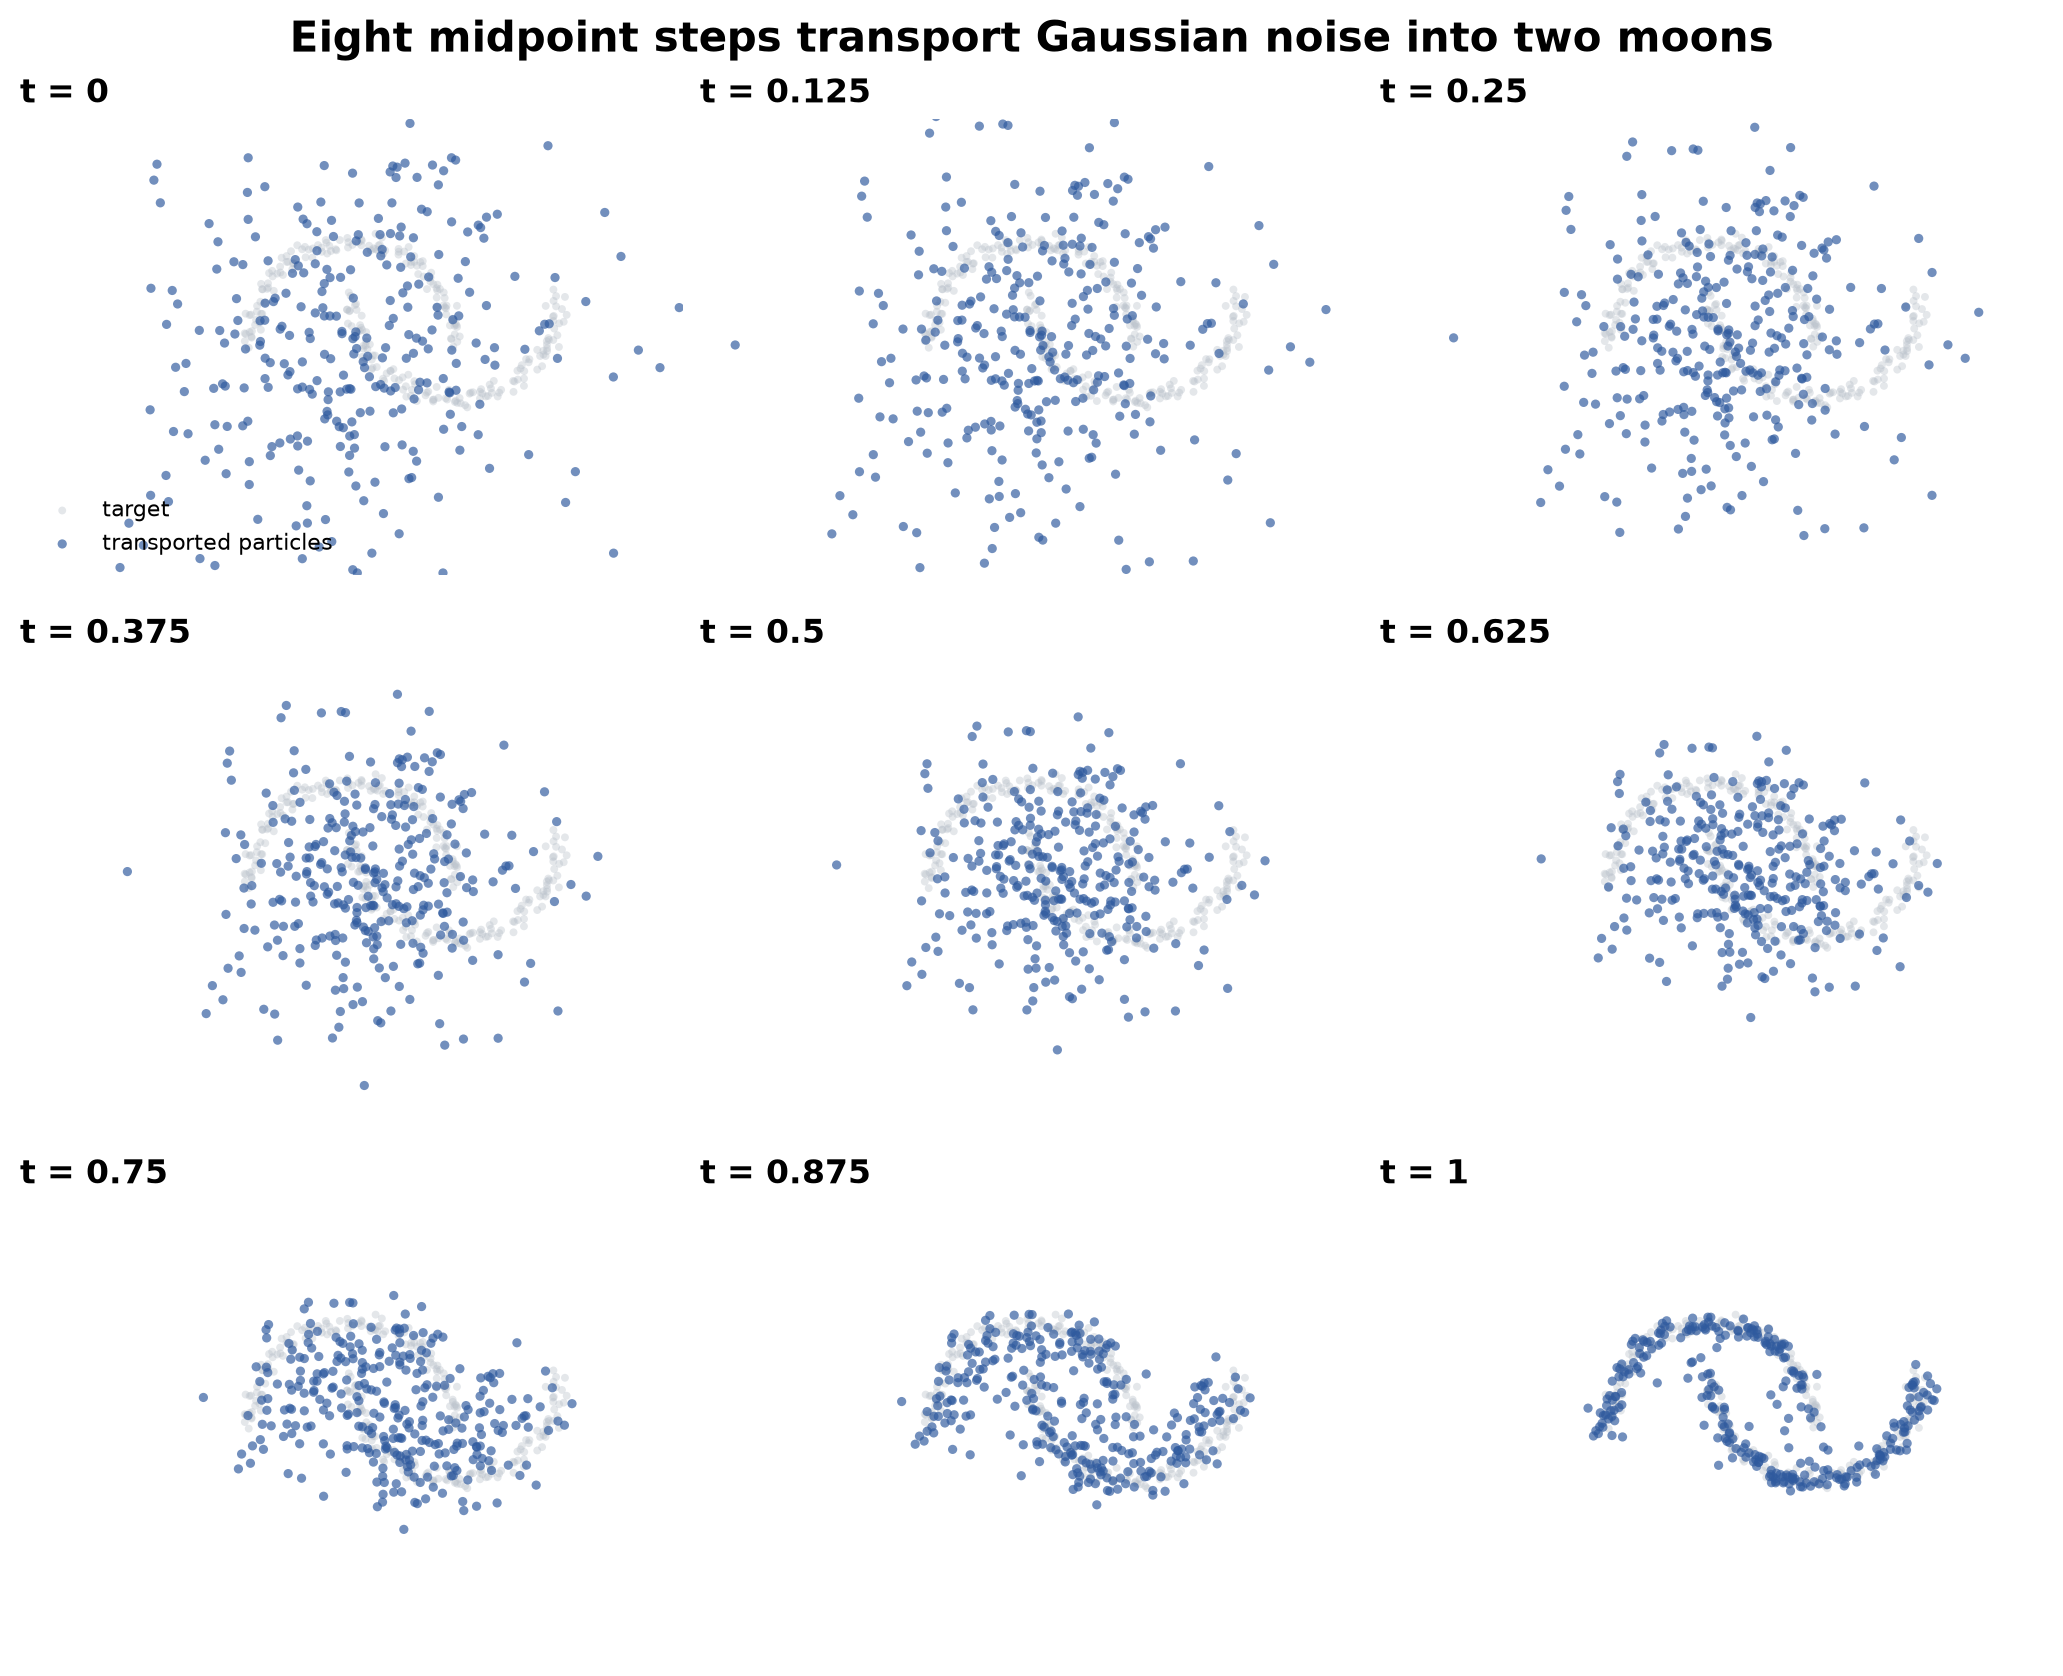
\includegraphics[width=0.91\linewidth]{two_moons_flow_path.png}
\caption{A common set of particles evolves from an isotropic Gaussian into the
two-moons geometry. Gray points are the target reference at every time, so shape
formation is directly visible rather than inferred from a scalar metric.}
\end{figure}

On fixed evaluation draws, RBF MMD$^2$ was 0.00076;
84.0\% of generated points fell within
the support threshold defined by the 95th percentile held-out-to-reference nearest
distance. The generated median nearest-reference distance was
0.0175, versus
0.0161 for an independent held-out draw.
These values and the plot establish a fixed-seed pipeline/geometric demonstration,
not general superiority of flow matching.

\subsection*{4.6 The same two moons expose the VAE tradeoff}

The VAE uses the same 256 noisy two-moons observations. Its encoder and decoder
are width-64 ELU PyTorch MLPs, its latent dimension is two, and
$q_\phi(z\mid x)$ is diagonal Gaussian. The decoder likelihood is
$\mathcal N(\mu_\theta(z),0.05^2I)$. Training ran for 2,500 epochs with Adam at
$10^{-3}$; generation uses one prior draw and one decoder evaluation.

\begin{figure}[H]
\centering
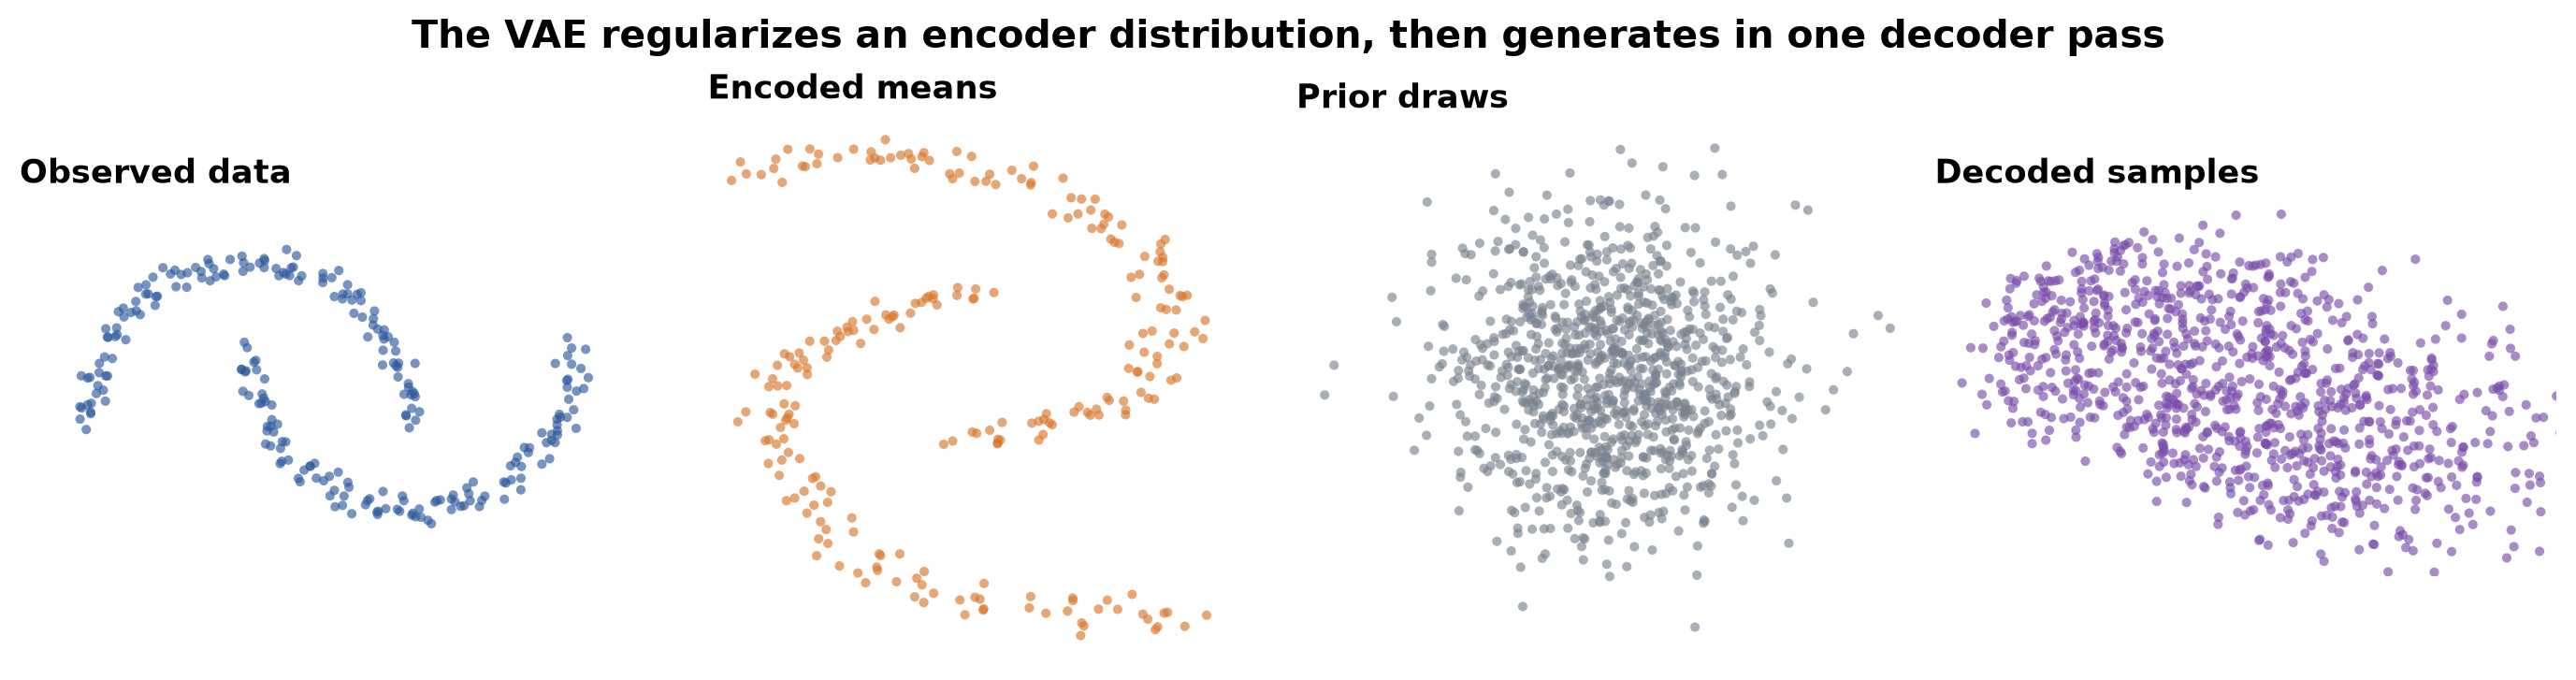
\includegraphics[width=0.98\linewidth]{two_moons_vae.png}
\caption{Observed points, posterior means, standard-normal prior draws, and
one-pass decoded samples. The encoded means form two thin curves, but prior mass
also occupies the region between them. The decoder maps that mass into a smooth
bridge rather than preserving the target's empty gap.}
\end{figure}

Held-out reconstruction MSE was $2.35\times10^{-4}$ and the mean posterior KL
was $4.782$ nats. Those apparently favorable training diagnostics did not ensure
faithful prior samples: sample MMD$^2$ was $0.00305$, median nearest-reference
distance was $0.0906$ versus $0.0161$ for held-out data, and only $31.5\%$ of
samples fell inside the held-out support threshold. The flow demonstration
reached $84.0\%$ under the same support definition, but used repeated
vector-field evaluations. This fixed-seed contrast isolates a genuine tradeoff:
one-pass decoding and useful latent inference do not guarantee preservation of a
thin multimodal manifold.


\section*{5. Diffusion and score-based modeling}

For a variance-preserving discrete diffusion,
\[
 q(x_t\mid x_0)=\mathcal N(\sqrt{\bar\alpha_t}x_0,
 (1-\bar\alpha_t)I),\qquad
 x_t=\sqrt{\bar\alpha_t}x_0+\sqrt{1-\bar\alpha_t}\epsilon.
\]
The classroom model predicts the injected noise using
\[
 \mathcal L_\epsilon(\theta)=
 \E_{t,x_0,\epsilon}\lVert\epsilon-\epsilon_\theta(x_t,t)\rVert_2^2.
\]
This is connected to the weighted variational objective and denoising score
matching in DDPM \cite{ho2020ddpm}. In continuous time, a forward SDE that adds
noise has a reverse-time SDE whose drift depends on the score
$\nabla_x\log p_t(x)$; an associated probability-flow ODE shares the same
marginals \cite{song2021sde}. Thus diffusion and flow methods can share network
parameterizations and deterministic ODE samplers while differing in path,
regression target, weighting, and stochasticity.

The benchmark uses a linear 50-step beta schedule and deterministic DDIM-style
updates ($\eta=0$). This makes network-evaluation cost explicit and keeps sampling
reproducible. It omits U-Nets, attention, latent autoencoders, classifier-free
guidance, and high-resolution training; those are extensions after the mathematical
core is auditable.

\subsection*{5.1 Deriving the closed-form forward marginal}

\textbf{Model-preservation note.} The following derivations keep the exact
classroom choice above: a variance-preserving discrete diffusion, a linear
$\beta_t$ schedule, $\epsilon$-prediction, and deterministic DDIM-style
sampling with $\eta=0$. No experimental objective or sampler is replaced.

The one-step forward Markov kernel of a DDPM is
\cite{ho2020ddpm}
\[
 q(x_t\mid x_{t-1})
 =\mathcal N(\sqrt{\alpha_t}\,x_{t-1},\beta_t I),
 \qquad \alpha_t:=1-\beta_t.
\]
Equivalently,
\[
 x_t=\sqrt{\alpha_t}\,x_{t-1}+\sqrt{\beta_t}\,\epsilon_t,
 \qquad \epsilon_t\sim\mathcal N(0,I).
\]
Let $\bar\alpha_t=\prod_{s=1}^t\alpha_s$. Suppose inductively that
\[
 x_{t-1}
 =\sqrt{\bar\alpha_{t-1}}\,x_0
 +\sqrt{1-\bar\alpha_{t-1}}\,z,
 \qquad z\sim\mathcal N(0,I).
\]
Substitution into the one-step update gives
\begin{align*}
 x_t
 &=\sqrt{\alpha_t\bar\alpha_{t-1}}\,x_0\\
 &\quad+
 \sqrt{\alpha_t(1-\bar\alpha_{t-1})}\,z
 +\sqrt{\beta_t}\,\epsilon_t\\
 &=\sqrt{\bar\alpha_t}\,x_0+\xi_t.
\end{align*}
The last two terms are independent centered Gaussians. Their total covariance is
\begin{align*}
 \operatorname{Var}(\xi_t)
 &=\left[\alpha_t(1-\bar\alpha_{t-1})+\beta_t\right]I\\
 &=\left[\alpha_t-\bar\alpha_t+1-\alpha_t\right]I\\
 &=(1-\bar\alpha_t)I.
\end{align*}
Hence $\xi_t$ can be represented by one standard-normal draw,
\[
 \boxed{
 x_t=\sqrt{\bar\alpha_t}\,x_0
 +\sqrt{1-\bar\alpha_t}\,\epsilon,
 \qquad \epsilon\sim\mathcal N(0,I)
 }
\]
which yields the closed-form marginal already stated above. The practical
consequence is important: training can sample an arbitrary $t$ and construct
$x_t$ in one operation instead of simulating all $t$ preceding corruption
steps.

\subsection*{5.2 From the reverse posterior to the $\epsilon$-prediction loss}

The exact forward posterior conditioned on both $x_t$ and the clean sample
$x_0$ is Gaussian. Bayes' rule gives, up to a normalization constant,
\begin{align*}
 q(x_{t-1}\mid x_t,x_0)
 &\propto q(x_t\mid x_{t-1})q(x_{t-1}\mid x_0)\\
 &\propto
 \exp\Bigg\{-\frac{\|x_t-\sqrt{\alpha_t}x_{t-1}\|_2^2}{2\beta_t}
 -\frac{\|x_{t-1}-\sqrt{\bar\alpha_{t-1}}x_0\|_2^2}
 {2(1-\bar\alpha_{t-1})}\Bigg\}.
\end{align*}
Collecting the quadratic terms in $x_{t-1}$ gives precision
\begin{align*}
 A_t
 &=\frac{\alpha_t}{\beta_t}
   +\frac{1}{1-\bar\alpha_{t-1}}\\
 &=\frac{1-\bar\alpha_t}
 {\beta_t(1-\bar\alpha_{t-1})}.
\end{align*}
Therefore the posterior variance is
\[
 \boxed{
 \tilde\beta_t=A_t^{-1}
 =\frac{1-\bar\alpha_{t-1}}{1-\bar\alpha_t}\,\beta_t
 }.
\]
The linear term in the exponent is
\[
 B_t=\frac{\sqrt{\alpha_t}}{\beta_t}x_t
 +\frac{\sqrt{\bar\alpha_{t-1}}}{1-\bar\alpha_{t-1}}x_0,
\]
so completing the square yields
\begin{align*}
 \tilde\mu_t(x_t,x_0)
 &=A_t^{-1}B_t\\
 &=\frac{\sqrt{\bar\alpha_{t-1}}\beta_t}{1-\bar\alpha_t}x_0
 +\frac{\sqrt{\alpha_t}(1-\bar\alpha_{t-1})}{1-\bar\alpha_t}x_t.
\end{align*}
Now use the forward reparameterization
\[
 x_0=\frac{x_t-\sqrt{1-\bar\alpha_t}\,\epsilon}
 {\sqrt{\bar\alpha_t}}.
\]
After substitution and simplification,
\[
 \boxed{
 \tilde\mu_t(x_t,x_0)
 =\frac{1}{\sqrt{\alpha_t}}
 \left(x_t-
 \frac{\beta_t}{\sqrt{1-\bar\alpha_t}}\epsilon\right)
 }.
\]
This expression motivates parameterizing the learned reverse mean with a noise
predictor:
\[
 \mu_\theta(x_t,t)
 =\frac{1}{\sqrt{\alpha_t}}
 \left(x_t-
 \frac{\beta_t}{\sqrt{1-\bar\alpha_t}}
 \epsilon_\theta(x_t,t)\right).
\]
If the reverse covariance is fixed to $\sigma_t^2I$, then the Gaussian KL term
in the variational objective satisfies
\begin{align*}
 L_{t-1}
 &=\E\,D_{\rm KL}\!\left(
 q(x_{t-1}\mid x_t,x_0)\Vert p_\theta(x_{t-1}\mid x_t)
 \right)\\
 &=\E\left[
 \frac{1}{2\sigma_t^2}
 \|\tilde\mu_t-\mu_\theta\|_2^2\right]+C\\
 &=\E\left[
 \frac{\beta_t^2}
 {2\sigma_t^2\alpha_t(1-\bar\alpha_t)}
 \|\epsilon-\epsilon_\theta(x_t,t)\|_2^2\right]+C,
\end{align*}
where $C$ is independent of $\theta$ \cite{ho2020ddpm}. Thus the
$\epsilon$-MSE is not an arbitrary denoising heuristic: with a particular
$t$-dependent weight it is one term of the diffusion variational bound.

The classroom loss
\[
 \mathcal L_\epsilon
 =\E\|\epsilon-\epsilon_\theta(x_t,t)\|_2^2
\]
uses the common \emph{unweighted} simplified objective of DDPM. It deliberately
drops the coefficient above. Therefore it is best described as a reweighted
variational/denoising objective, not as numerically identical to the full ELBO.
This distinction clarifies what the benchmark is actually optimizing without
changing its implementation.

\subsection*{5.3 $\epsilon$, $x_0$, score, and velocity parameterizations}

Write
\[
 a_t:=\sqrt{\bar\alpha_t},\qquad
 b_t:=\sqrt{1-\bar\alpha_t},\qquad
 a_t^2+b_t^2=1.
\]
The forward relation is simply
\[
 x_t=a_tx_0+b_t\epsilon.
\]
Any two of $(x_t,x_0,\epsilon)$ determine the third:
\[
 \boxed{\quad
 \epsilon=\frac{x_t-a_tx_0}{b_t},\qquad
 x_0=\frac{x_t-b_t\epsilon}{a_t}.
 \quad}
\]
For the conditional Gaussian $q(x_t\mid x_0)$,
\begin{align*}
 \nabla_{x_t}\log q(x_t\mid x_0)
 &=-\frac{x_t-a_tx_0}{b_t^2}\\
 &=-\frac{\epsilon}{b_t}.
\end{align*}
After averaging over $x_0$ conditional on $x_t$, the population-optimal noise
predictor therefore determines the marginal score through
\[
 s_t(x_t)=\nabla_{x_t}\log q_t(x_t)
 =-\frac{\E[\epsilon\mid x_t]}{b_t}.
\]
This is the algebraic bridge between noise prediction and score prediction.

A commonly used velocity-like parameterization for variance-preserving
diffusion is \cite{salimans2022distill}
\[
 v_t=a_t\epsilon-b_tx_0.
\]
Together with $x_t=a_tx_0+b_t\epsilon$, this is an orthogonal rotation:
\[
 \begin{bmatrix}x_t\\v_t\end{bmatrix}
 =
 \begin{bmatrix}a_t&b_t\\-b_t&a_t\end{bmatrix}
 \begin{bmatrix}x_0\\\epsilon\end{bmatrix}.
\]
Hence the inverse formulas are particularly clean:
\[
 \boxed{
 x_0=a_tx_t-b_tv_t,\qquad
 \epsilon=b_tx_t+a_tv_t.
 }
\]
These formulas explain why papers and software may describe apparently
different $x_0$-, $\epsilon$-, score-, or $v$-prediction networks while still
parameterizing the same underlying denoising information. The present benchmark
continues to train $\epsilon_\theta$; the other forms are included only to make
that choice interpretable.

\subsection*{5.4 The deterministic DDIM update used by the benchmark}

The DDIM construction uses the same trained denoiser as DDPM but permits a
non-Markovian sampling process and a reduced set of time indices
\cite{song2021ddim}. Let $s<t$ be two consecutive times selected by the sampler.
From the network prediction at time $t$, first reconstruct
\[
 \hat x_0
 =\frac{x_t-b_t\epsilon_\theta(x_t,t)}{a_t}.
\]
For the deterministic choice $\eta=0$, DDIM takes
\[
 \boxed{
 x_s=a_s\hat x_0+b_s\epsilon_\theta(x_t,t)
 }.
\]
Substituting the expression for $\hat x_0$ makes the update completely explicit:
\begin{align*}
 x_s
 &=\frac{a_s}{a_t}
 \big(x_t-b_t\epsilon_\theta(x_t,t)\big)
 +b_s\epsilon_\theta(x_t,t)\\
 &=\frac{a_s}{a_t}x_t
 +\left(b_s-\frac{a_sb_t}{a_t}\right)
 \epsilon_\theta(x_t,t).
\end{align*}
There is no fresh Gaussian draw in this $\eta=0$ update. Once the initial
$x_T$ and the time grid are fixed, the trajectory is deterministic. This is the
specific reason the benchmark can report one network evaluation per selected
diffusion step and obtain reproducible sampling for a fixed initial noise draw.
It also explains why using 5, 10, 20, or 50 selected times changes the numerical
sampling path without retraining the denoiser. The DDIM formulation likewise identifies $\eta=0$ as the deterministic setting
\cite{song2021ddim}.

\subsection*{5.5 Why the probability-flow ODE has the factor $1/2$}

The connection between diffusion and deterministic flow can be seen directly
from the Fokker--Planck equation. For the forward SDE
\[
 dX=f(X,t)\,dt+g(t)\,dW_t,
\]
the density evolves as
\[
 \partial_t p_t
 =-\nabla\!\cdot(f p_t)+\frac12g(t)^2\Delta p_t.
\]
Use
\[
 \Delta p_t
 =\nabla\!\cdot(\nabla p_t)
 =\nabla\!\cdot\big(p_t\nabla\log p_t\big).
\]
Then
\begin{align*}
 \partial_t p_t
 &=-\nabla\!\cdot(f p_t)
 +\frac12g(t)^2
 \nabla\!\cdot\big(p_t\nabla\log p_t\big)\\
 &=-\nabla\!\cdot\left(
 \left[f-\frac12g(t)^2\nabla\log p_t\right]p_t
 \right).
\end{align*}
The last line is a continuity equation. Therefore the deterministic ODE
\[
 \boxed{
 \frac{dX}{dt}
 =f(X,t)-\frac12g(t)^2\nabla_x\log p_t(X)
 }
\]
produces the same one-time marginals as the forward SDE, under the regularity
conditions needed for the corresponding equations to be well posed
\cite{song2021sde}. This derivation explains the factor $1/2$ in the
probability-flow ODE. The reverse-time SDE instead uses the full
$g(t)^2\nabla\log p_t$ correction because it still contains a stochastic
diffusion term. Equal marginals do not imply equal individual trajectories.

\section*{6. Reusable implementation and controlled comparison}

The repository separates reusable models from orchestration. Neural-network
primitives are not reimplemented. Flow and diffusion use time-conditioned
\code{nn.Module} regressors with standard \code{Linear} and activation layers.
The VAE uses standard PyTorch encoders, posterior heads, decoders, convolutional
layers, binary cross-entropy, and the analytic Gaussian KL. Every wrapper keeps
tensor shapes, minibatch loops, train/evaluation modes, validation, autograd, and
optimizer updates explicit \cite{pytorchDocs}.

The run requested device \code{auto}; every fitted architecture
reported resolved device \code{mps}. The command-line policy also
accepts \code{auto}, \code{cuda}, and \code{mps}. \code{auto} prefers
CUDA, then Apple Metal, then CPU; explicit unavailable accelerators raise an
error rather than silently changing hardware.

The controlled flow/diffusion comparison is an architecture ablation, not a
duplicate neural implementation. A two-hidden-layer tanh MLP is compared with a
single linear map under identical regression settings. The VAE is an additional
model-family comparison with a different objective and sampler; its row is not a
matched capacity intervention and its objective scale is not comparable to MSE.

\begin{table}[H]
\centering
\small
\begin{tabular}{llrrrrr}
\toprule
Family & Architecture & Epochs & Params & Train objective & Valid. objective & Fit sec. \\
\midrule
Flow matching & mlp & 100 & 5320 & 1.4003 & 1.4823 & 9.98 \\
Flow matching & linear ablation & 100 & 80 & 1.9687 & 1.9872 & 4.18 \\
Diffusion & mlp & 100 & 5320 & 0.6725 & 0.7313 & 9.76 \\
Diffusion & linear ablation & 100 & 80 & 0.8840 & 0.8949 & 4.31 \\
VAE & mlp encoder/decoder & 100 & 10644 & 11.7861 & 12.1028 & 4.03 \\
\bottomrule
\end{tabular}
\caption{PyTorch objective diagnostics. Flow/diffusion values are
per-coordinate MSE; VAE values are negative ELBO up to the fixed Gaussian
normalizing constant. Compare objectives within a family, not across rows.}
\end{table}

The normalizing-flow unit has a stricter numerical oracle. The affine flow's
change-of-variables log density agrees with SciPy's multivariate Gaussian to
maximum absolute gap 8.88e-15; its maximum
round-trip error is 8.88e-16, and forward/inverse
log determinants cancel to 0.00e+00. An
additional fixed Real-NVP-style coupling layer is unit-tested for exact inverse
and log-Jacobian cancellation \cite{dinh2017realnvp}.

\section*{7. Public-data protocol}

The empirical demonstration uses scikit-learn's 1,797-row copy of the UCI Optical
Recognition of Handwritten Digits data: 8-by-8 integer images with values 0--16,
ten digit classes, and no missing values. The UCI source assigns DOI
\href{https://doi.org/10.24432/C50P49}{10.24432/C50P49} and CC BY 4.0
licensing \cite{uciDigits}. A fixed stratified split has
1437 training and 360 held-out rows.

PCA is fitted \emph{only} on training images, uses whitening, and retains eight
components. The transformation is a declared capacity/compute choice, not an
innocent display operation. It retains 67.4\% of training variance,
and all training and evaluation occurs in that declared latent space. Therefore:

\begin{itemize}
\item decoded sample blur partly reflects discarded PCA information;
\item ``latent Fr\'echet distance'' compares Gaussian moments in this PCA space
and is not Inception-feature FID;
\item the fixed $k$-NN probe estimates digit diversity but is not a human fidelity
study; and
\item results validate code paths and expose tradeoffs; they do not rank modern
high-resolution architectures.
\end{itemize}


\subsection*{7.1 Original MNIST at native 28-by-28 resolution}

The second visual demonstration uses the original MNIST split: 60,000 training
and 10,000 test images at 28-by-28 resolution \cite{mnistOriginal}. All four
compressed IDX files are MD5-verified before parsing. The official distribution
page does not state an explicit dataset license, which is recorded rather than
silently replaced by a mirror's terms. The model uses all
60000 training rows.

The generator is class-conditional so students can see that a declared condition
changes the output distribution. A compact 95521-parameter
U-Net-style convolutional vector field is composed entirely from standard PyTorch
layers; the course code implements the flow target, optimization loop, exponential
moving average, and midpoint sampler explicitly. It trained for
8 epochs and sampled with 20
midpoint steps. The requested device was \code{auto}
and the resolved device was \code{mps}.

\begin{figure}[H]
\centering
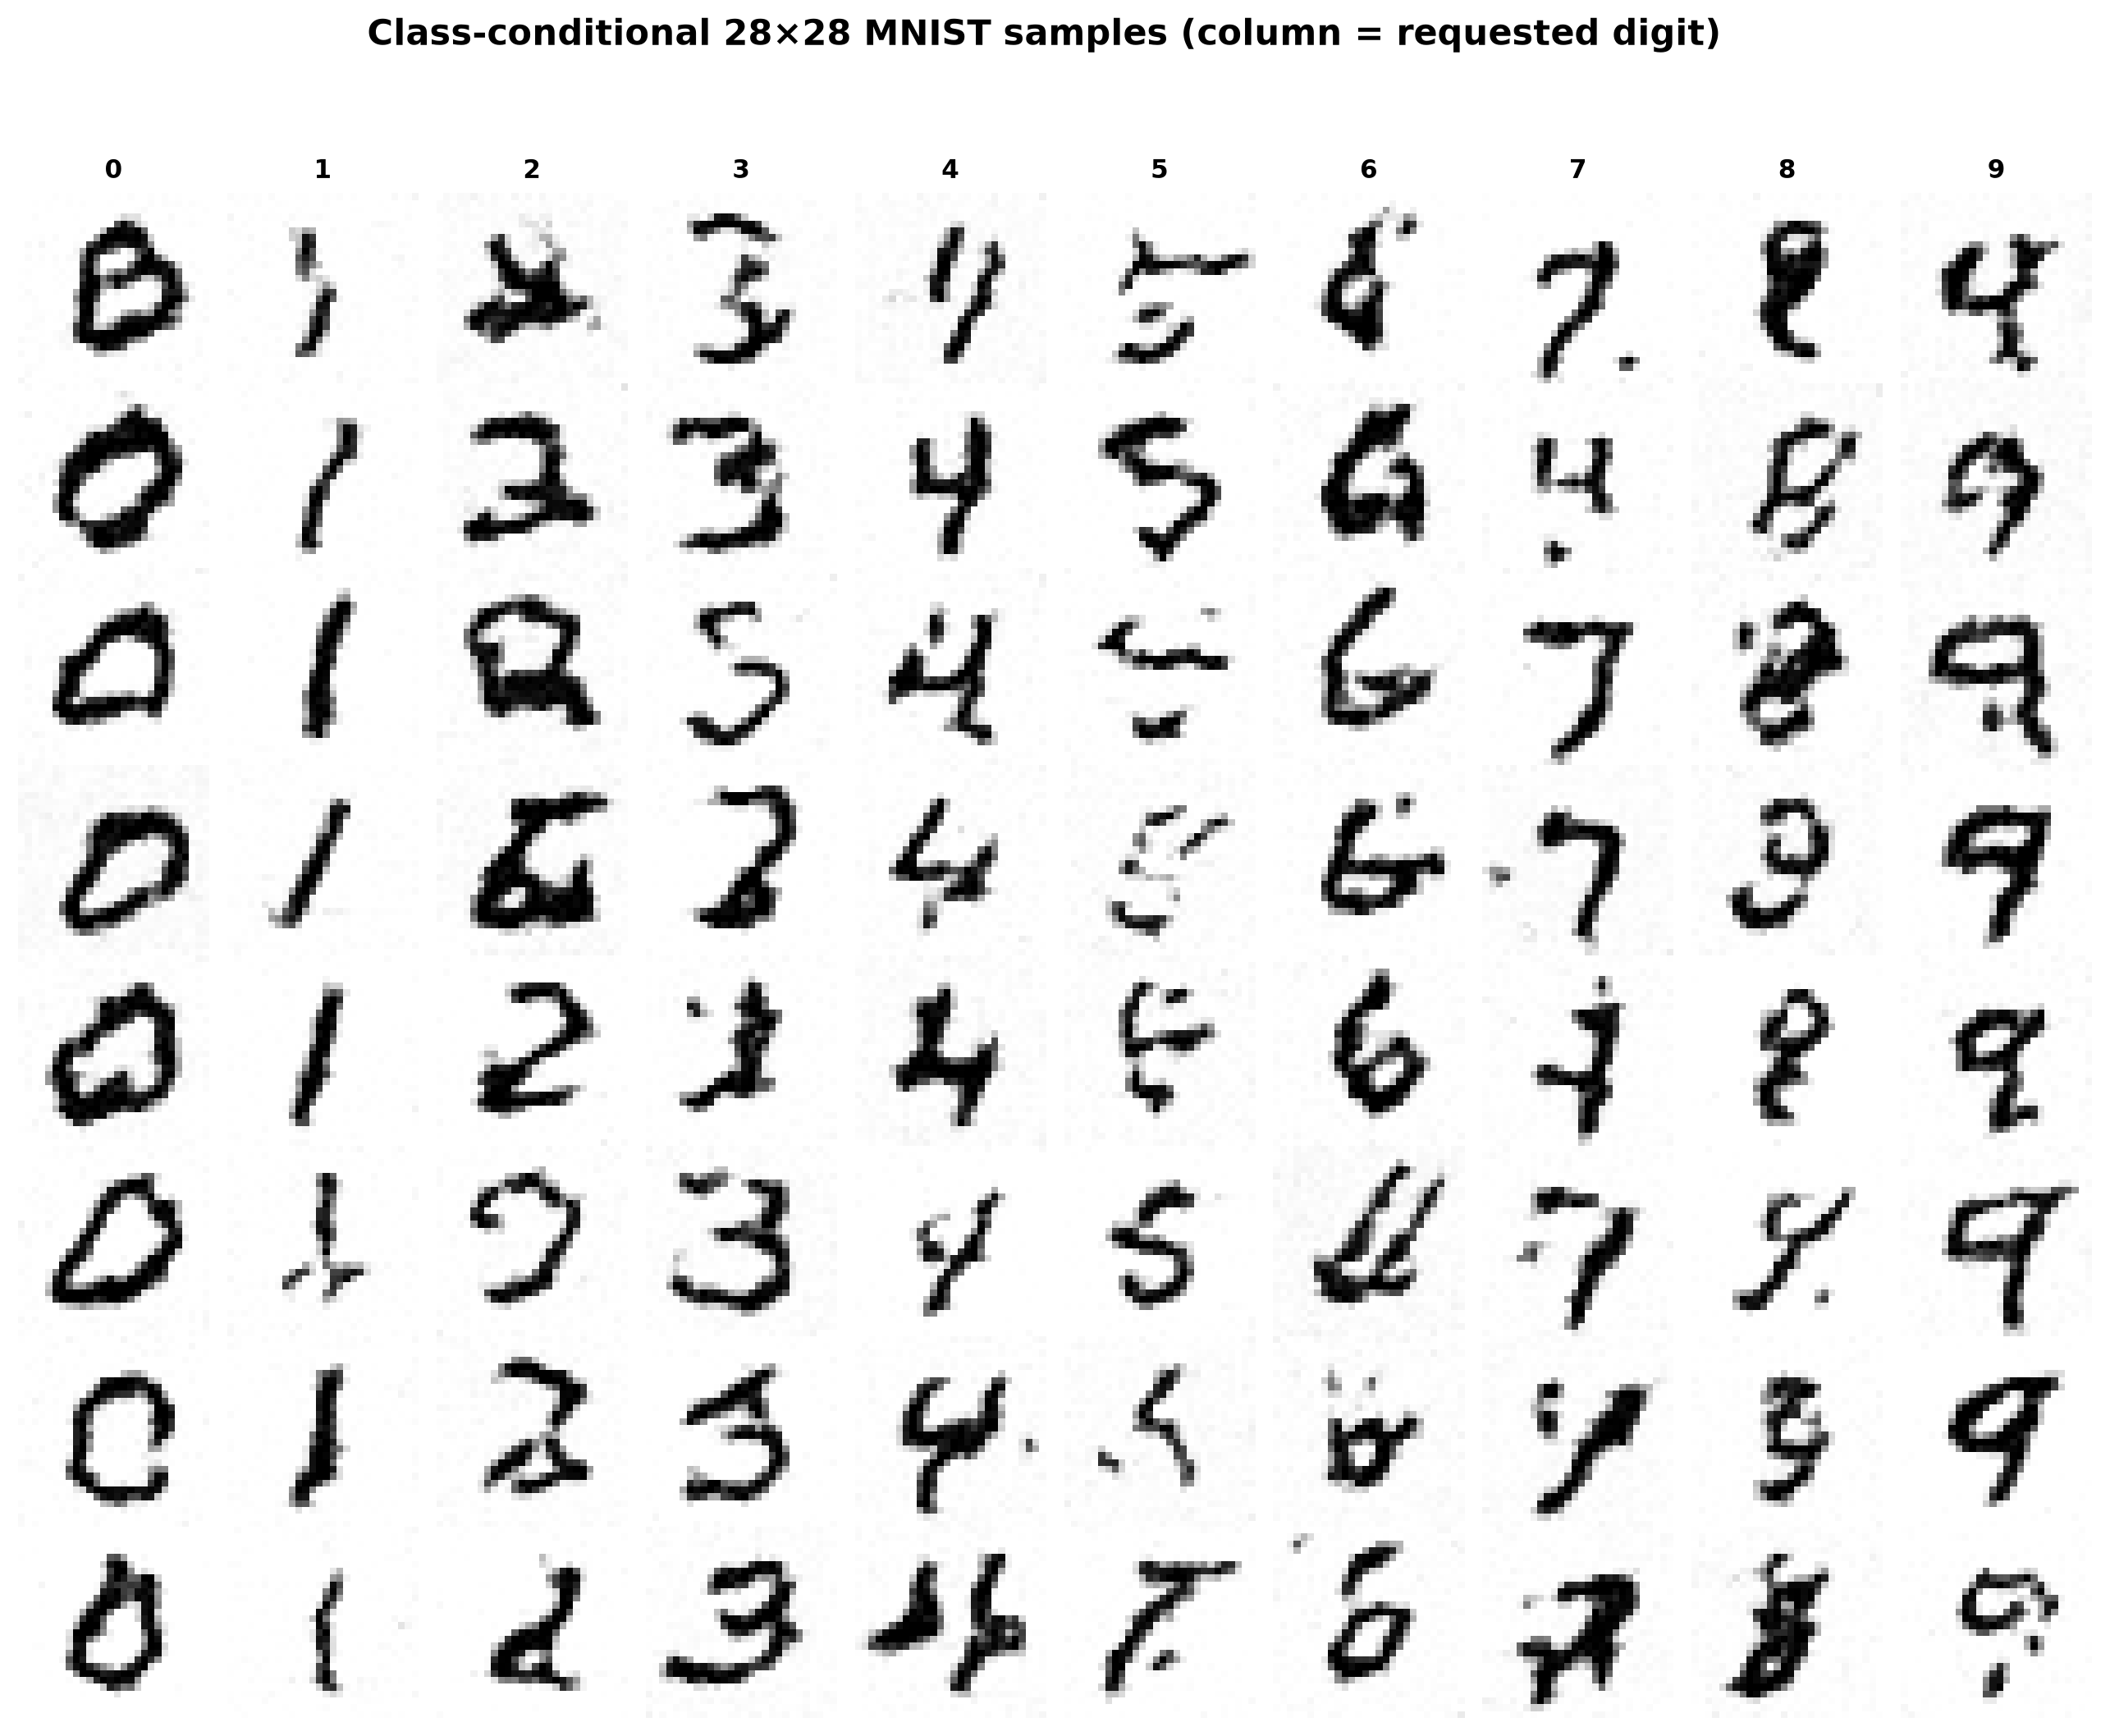
\includegraphics[width=0.93\linewidth]{mnist_28_generated.png}
\caption{Eighty generated 28-by-28 images. Columns 0--9 are requested class labels;
rows begin from independent Gaussian draws. This exposes both controllability and
within-label variation, including visible failures.}
\end{figure}

\begin{figure}[H]
\centering
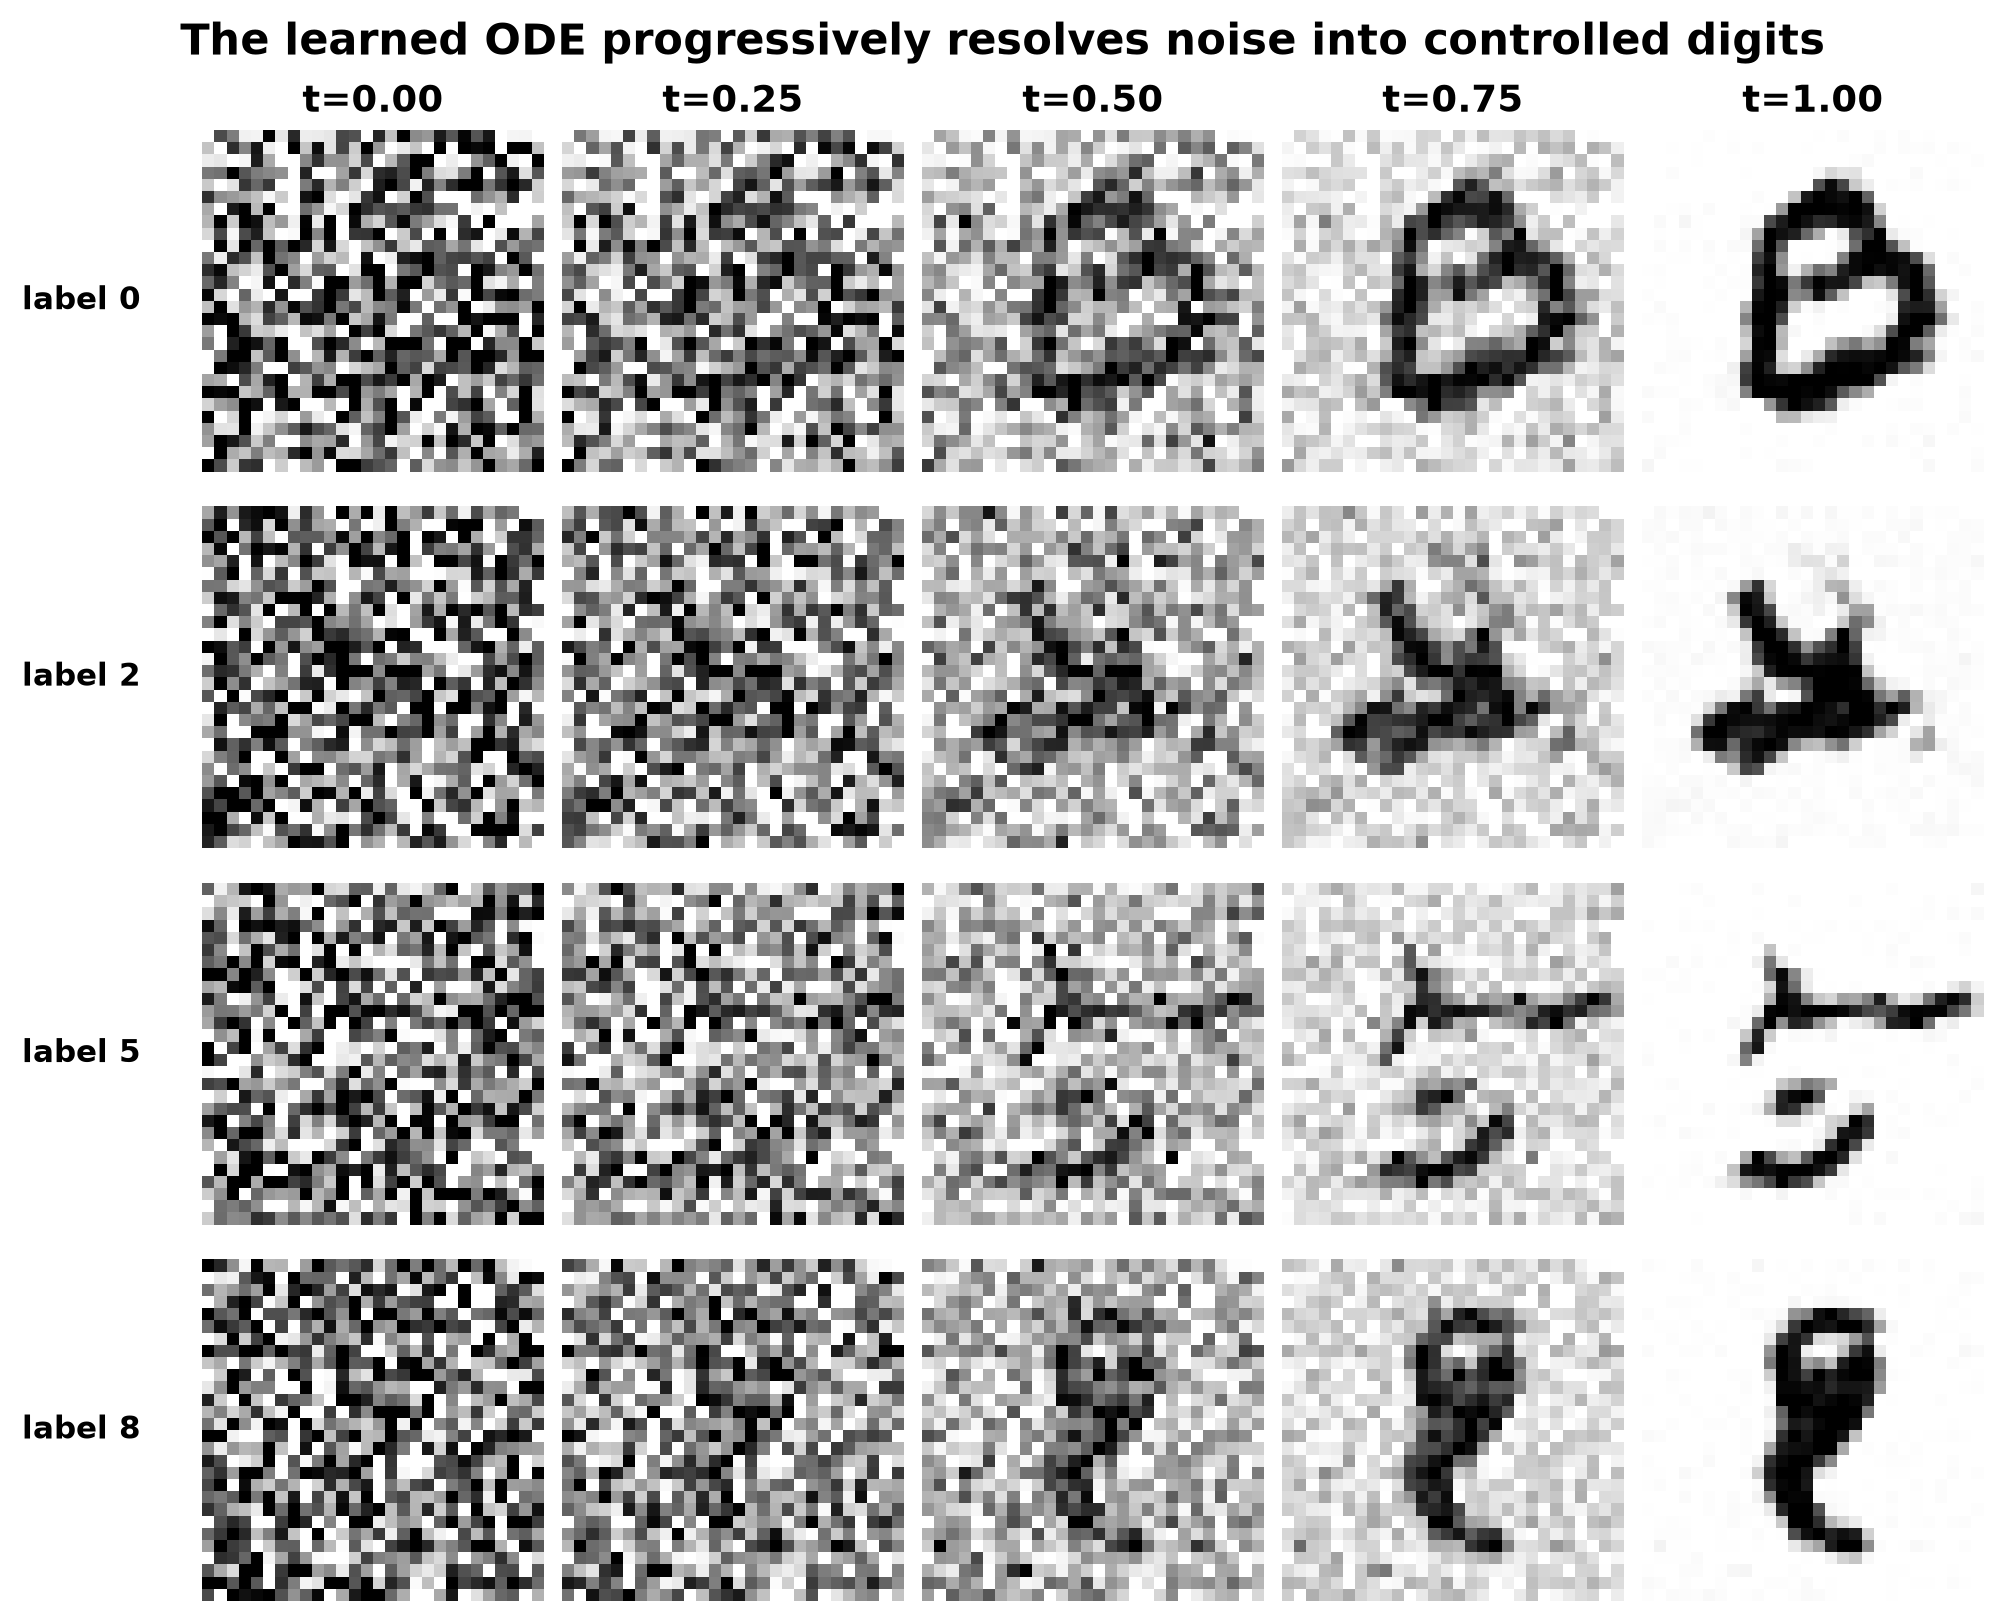
\includegraphics[width=0.86\linewidth]{mnist_28_flow_progression.png}
\caption{Selected particles along one 20-step midpoint trajectory. Global digit
structure and background suppression emerge continuously from noise.}
\end{figure}

\begin{figure}[H]
\centering
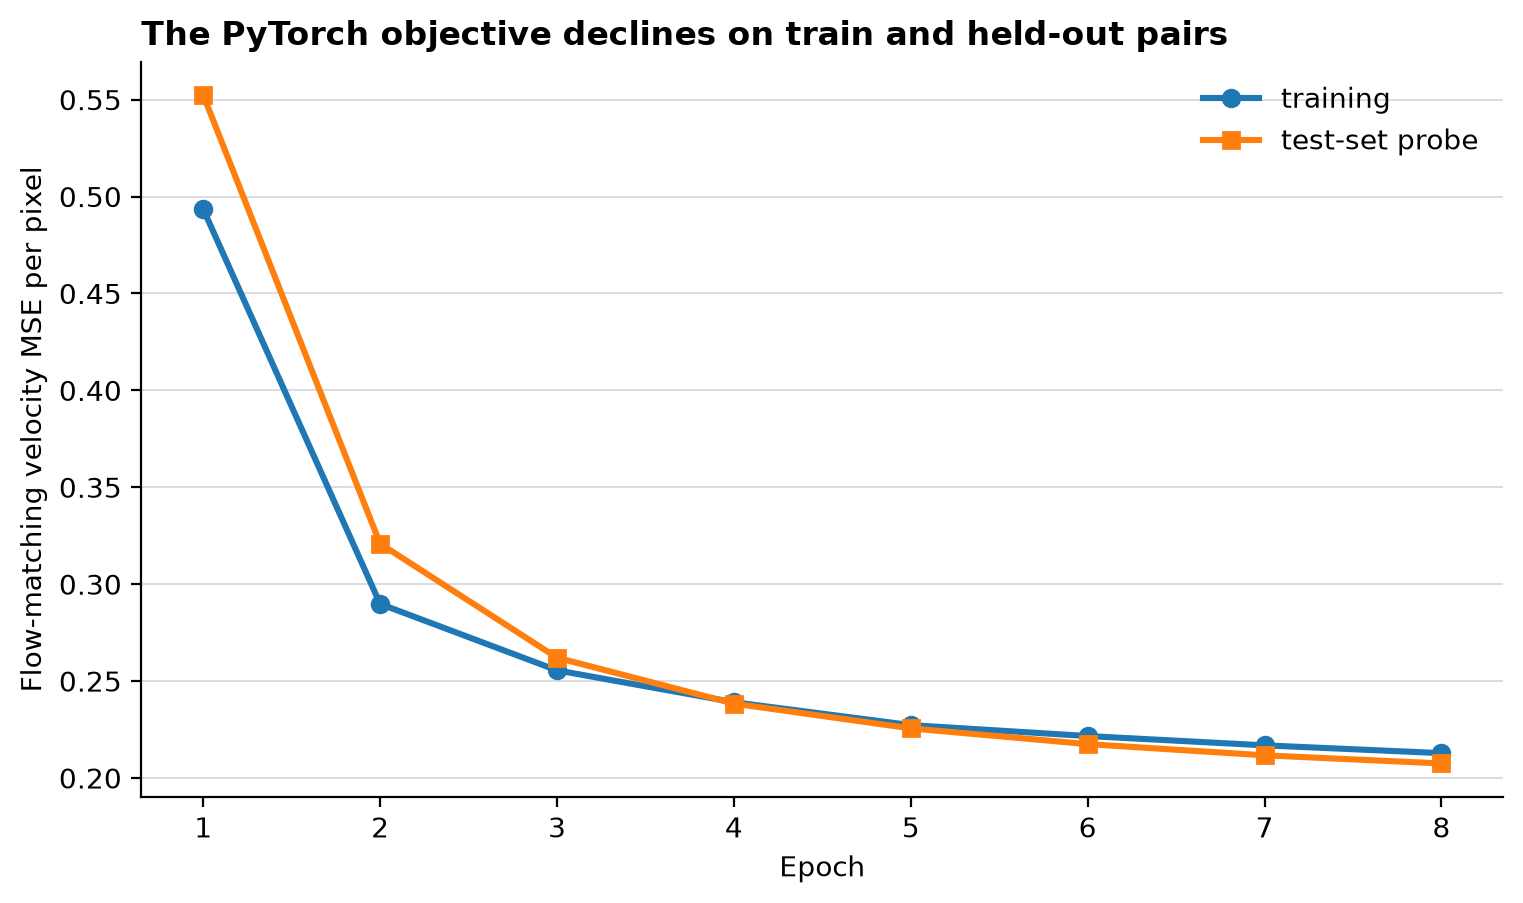
\includegraphics[width=0.78\linewidth]{mnist_28_training_curve.png}
\caption{Online flow-matching MSE per pixel. The held-out curve uses fixed noise/time
pairs over 2,000 official test images and is an objective diagnostic, not a sample-
quality metric.}
\end{figure}

Final training and held-out velocity MSE were
0.213 and
0.207. A 3-neighbor probe trained on 20,000
downsampled training images scored 95.5\%
on 2,000 original test images, then agreed with requested labels for
80.0\% of generated samples.
The probe makes conditional failures countable but is not human judgment or FID.
Generated median nearest-training distance was
2.398, compared with
1.797 for held-out images in the same
14-by-14 feature space; this does not indicate exact copying, but it is not a
privacy audit.

\subsection*{7.2 A conditional convolutional VAE on the same MNIST split}

The VAE uses the identical 60,000/10,000 MNIST split and one-hot label condition,
but a different probabilistic contract. The convolutional encoder returns a
16-dimensional diagonal Gaussian $q_\phi(z\mid x,y)$; the convolutional decoder
models independent Bernoulli pixels $p_\theta(x\mid z,y)$. The 430,337 parameters
belong to standard PyTorch convolution, transposed-convolution, normalization,
activation, and linear layers. Generation draws $z\sim\mathcal N(0,I)$ and uses
one decoder evaluation.

\begin{figure}[H]
\centering
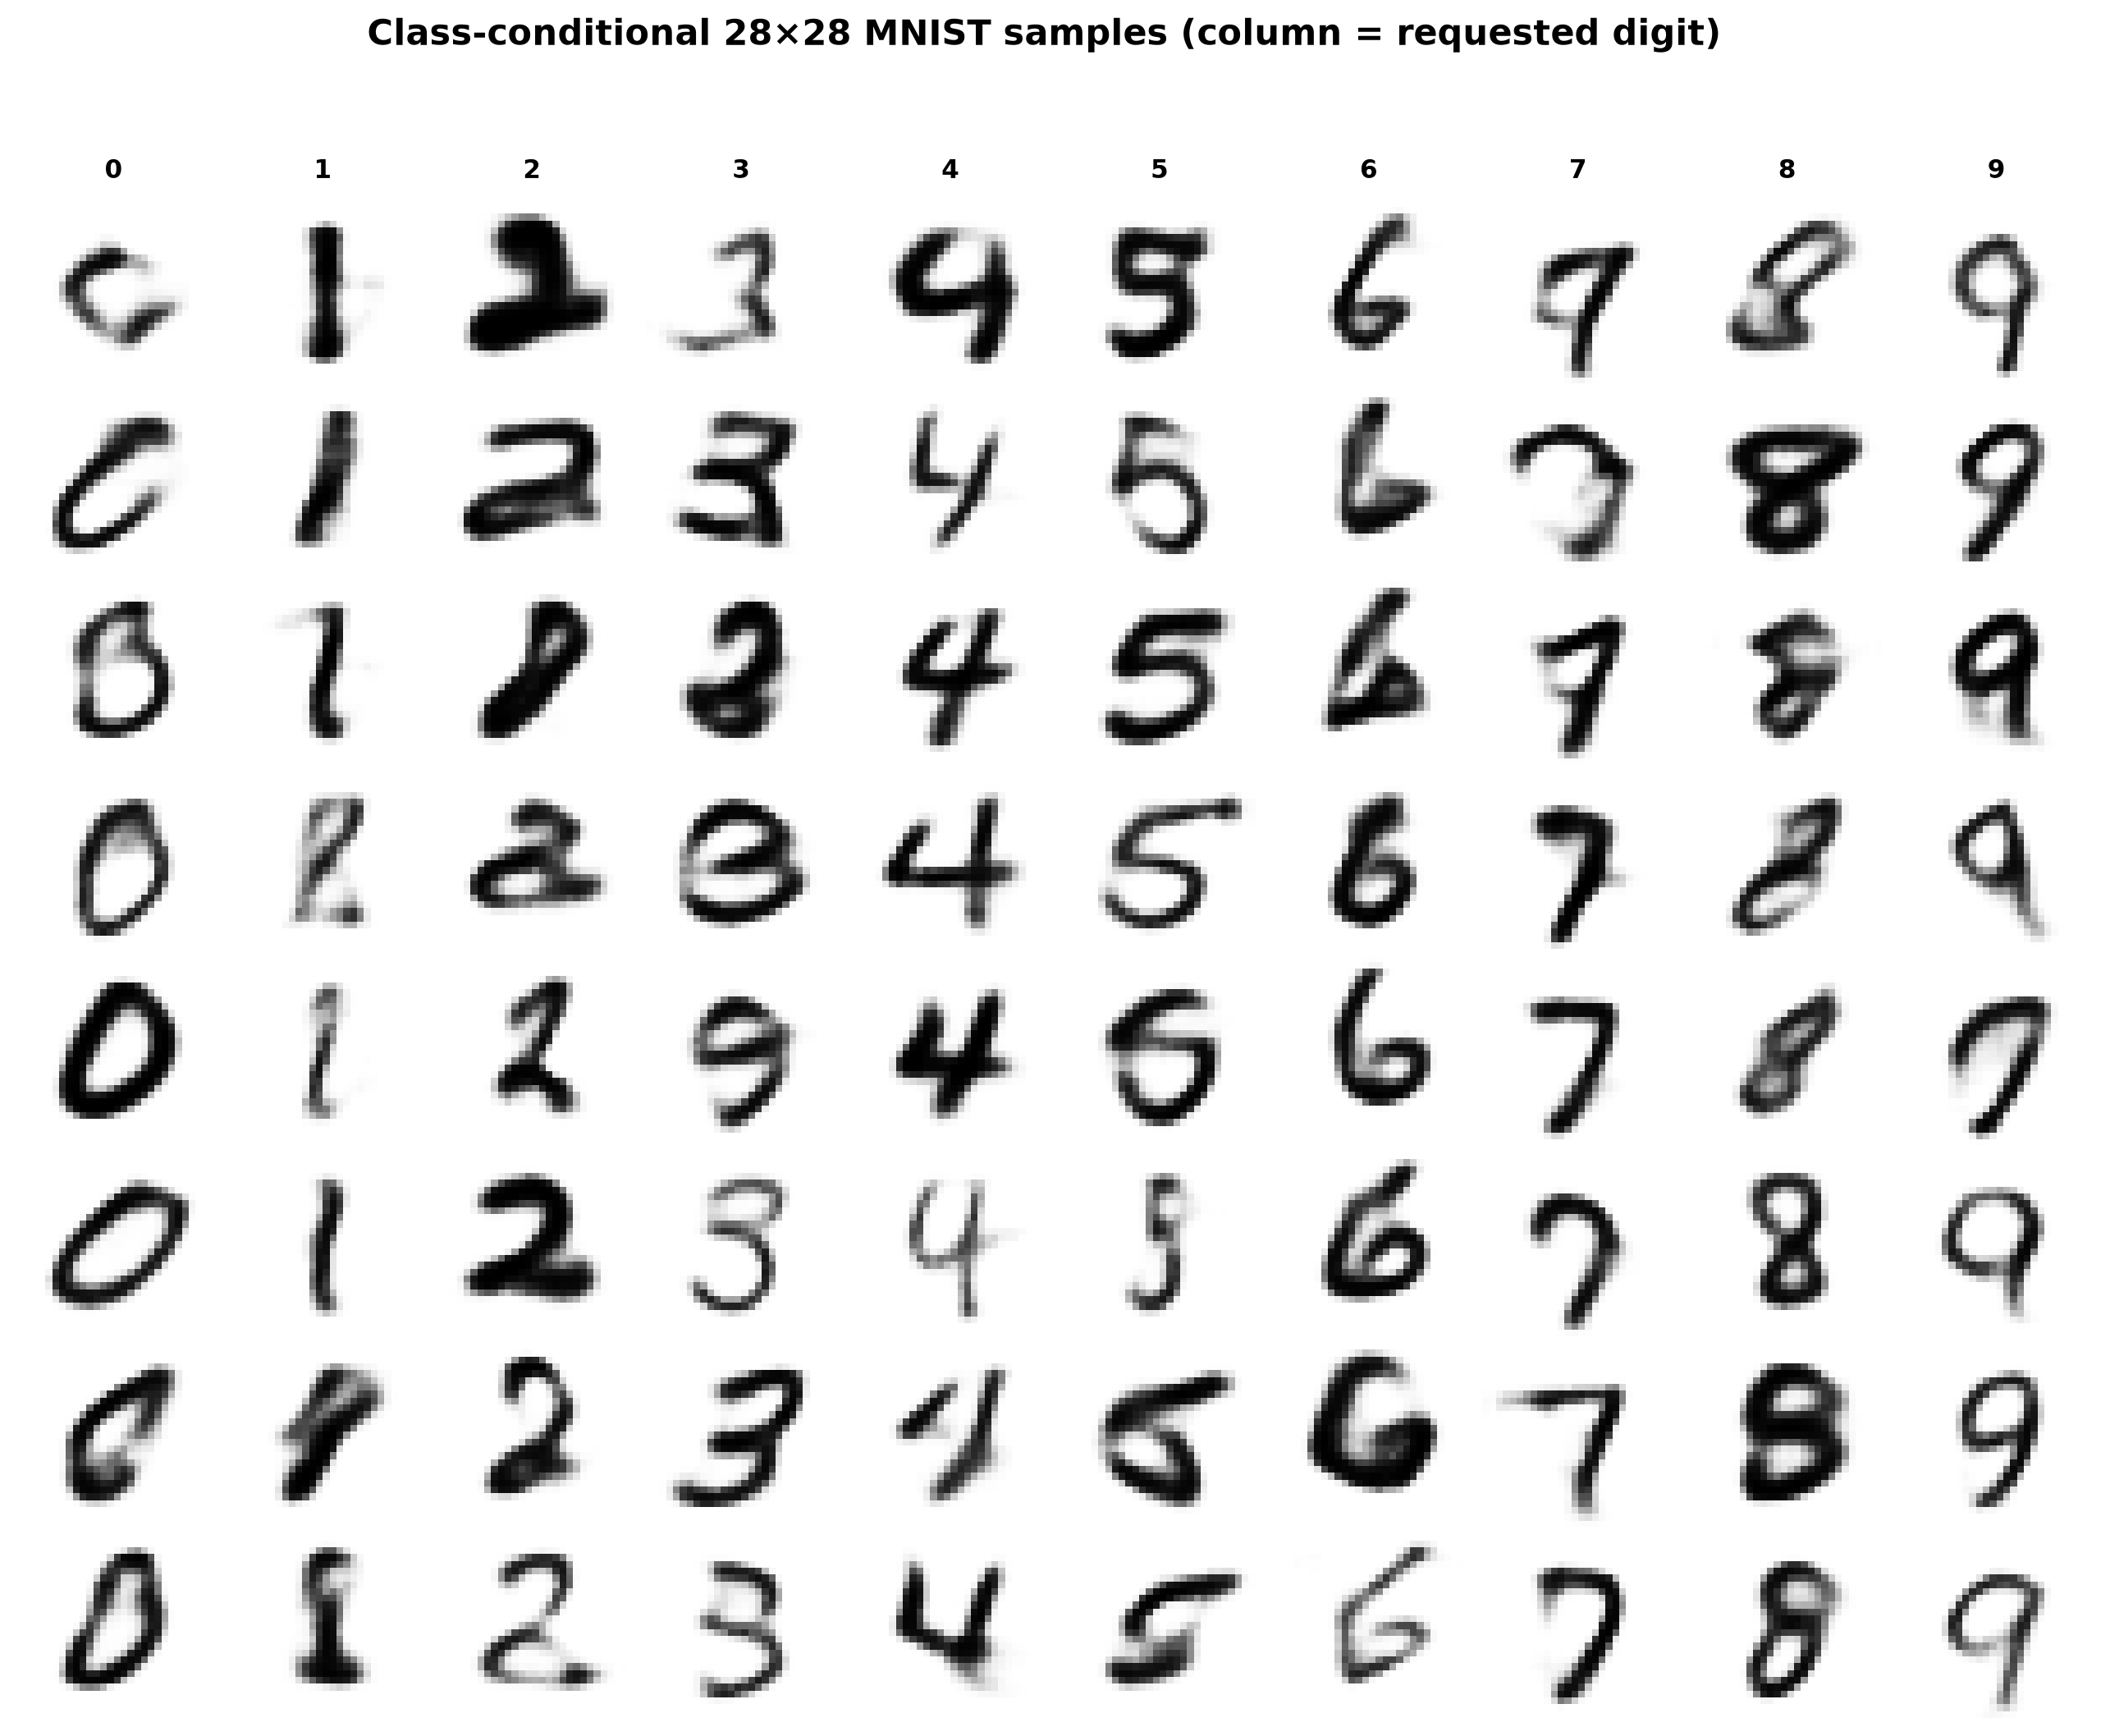
\includegraphics[width=0.93\linewidth]{mnist_28_vae_generated.png}
\caption{Eighty conditional VAE samples. Columns identify requested digits and
rows use independent prior draws. The one-pass samples are recognizable but
smoother than many flow outputs; ambiguous samples are retained rather than
curated away.}
\end{figure}

\begin{figure}[H]
\centering
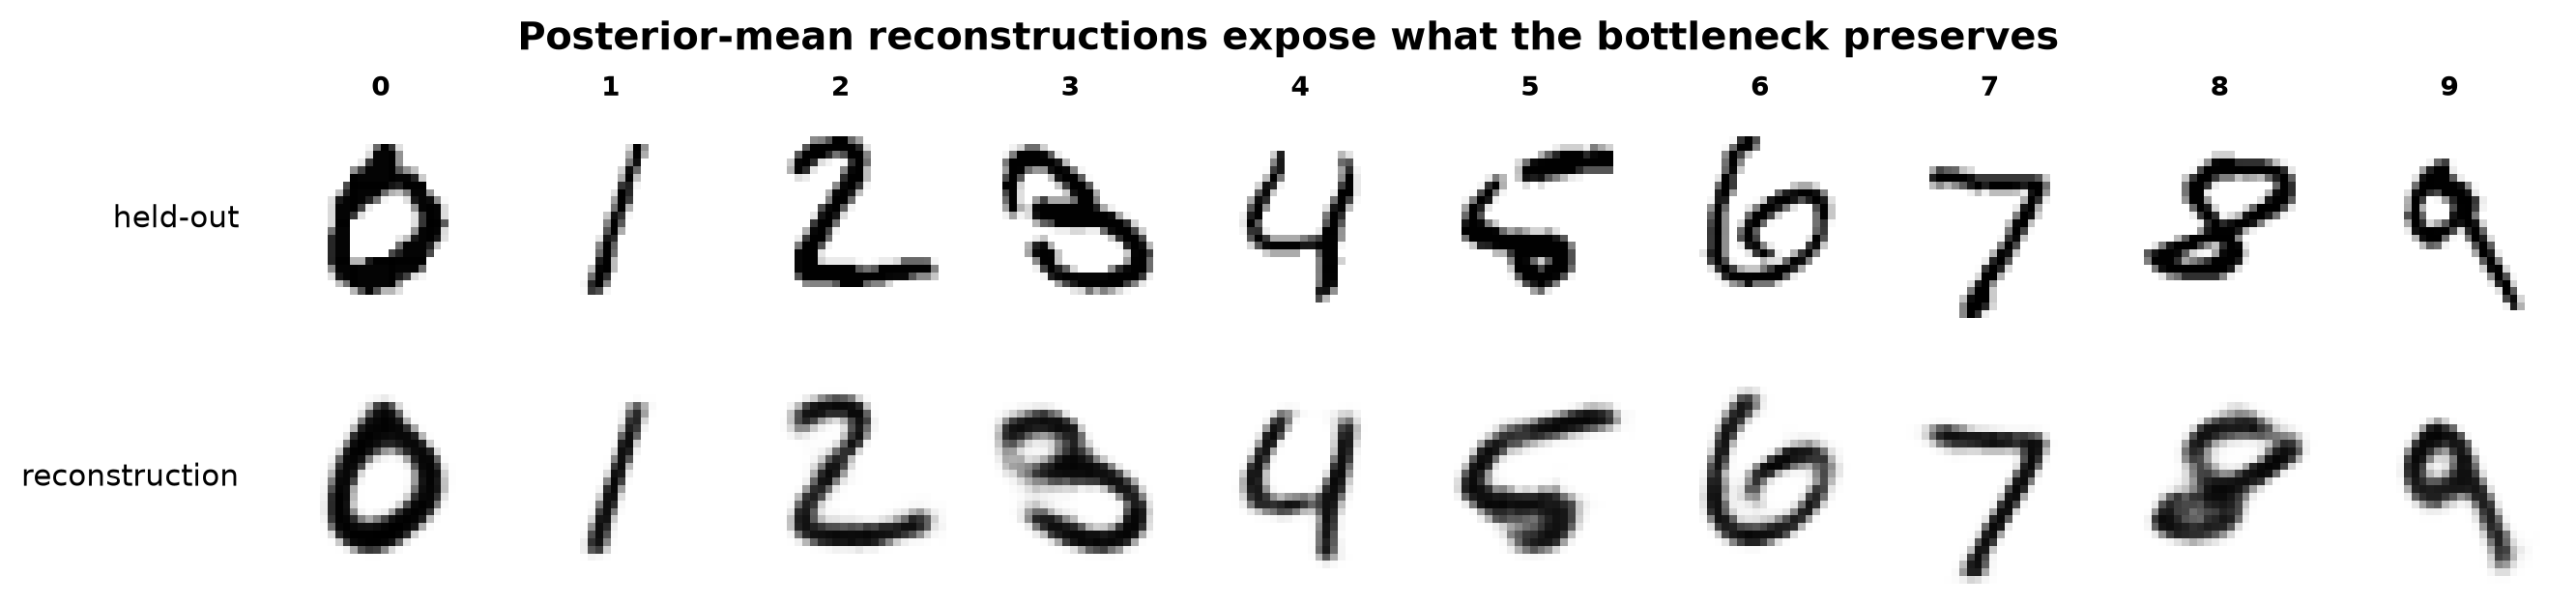
\includegraphics[width=0.94\linewidth]{mnist_28_vae_reconstruction.png}
\caption{One held-out image per class and its posterior-mean reconstruction.
This tests the encoder-decoder information path, not the prior-sampling path.}
\end{figure}

\begin{figure}[H]
\centering
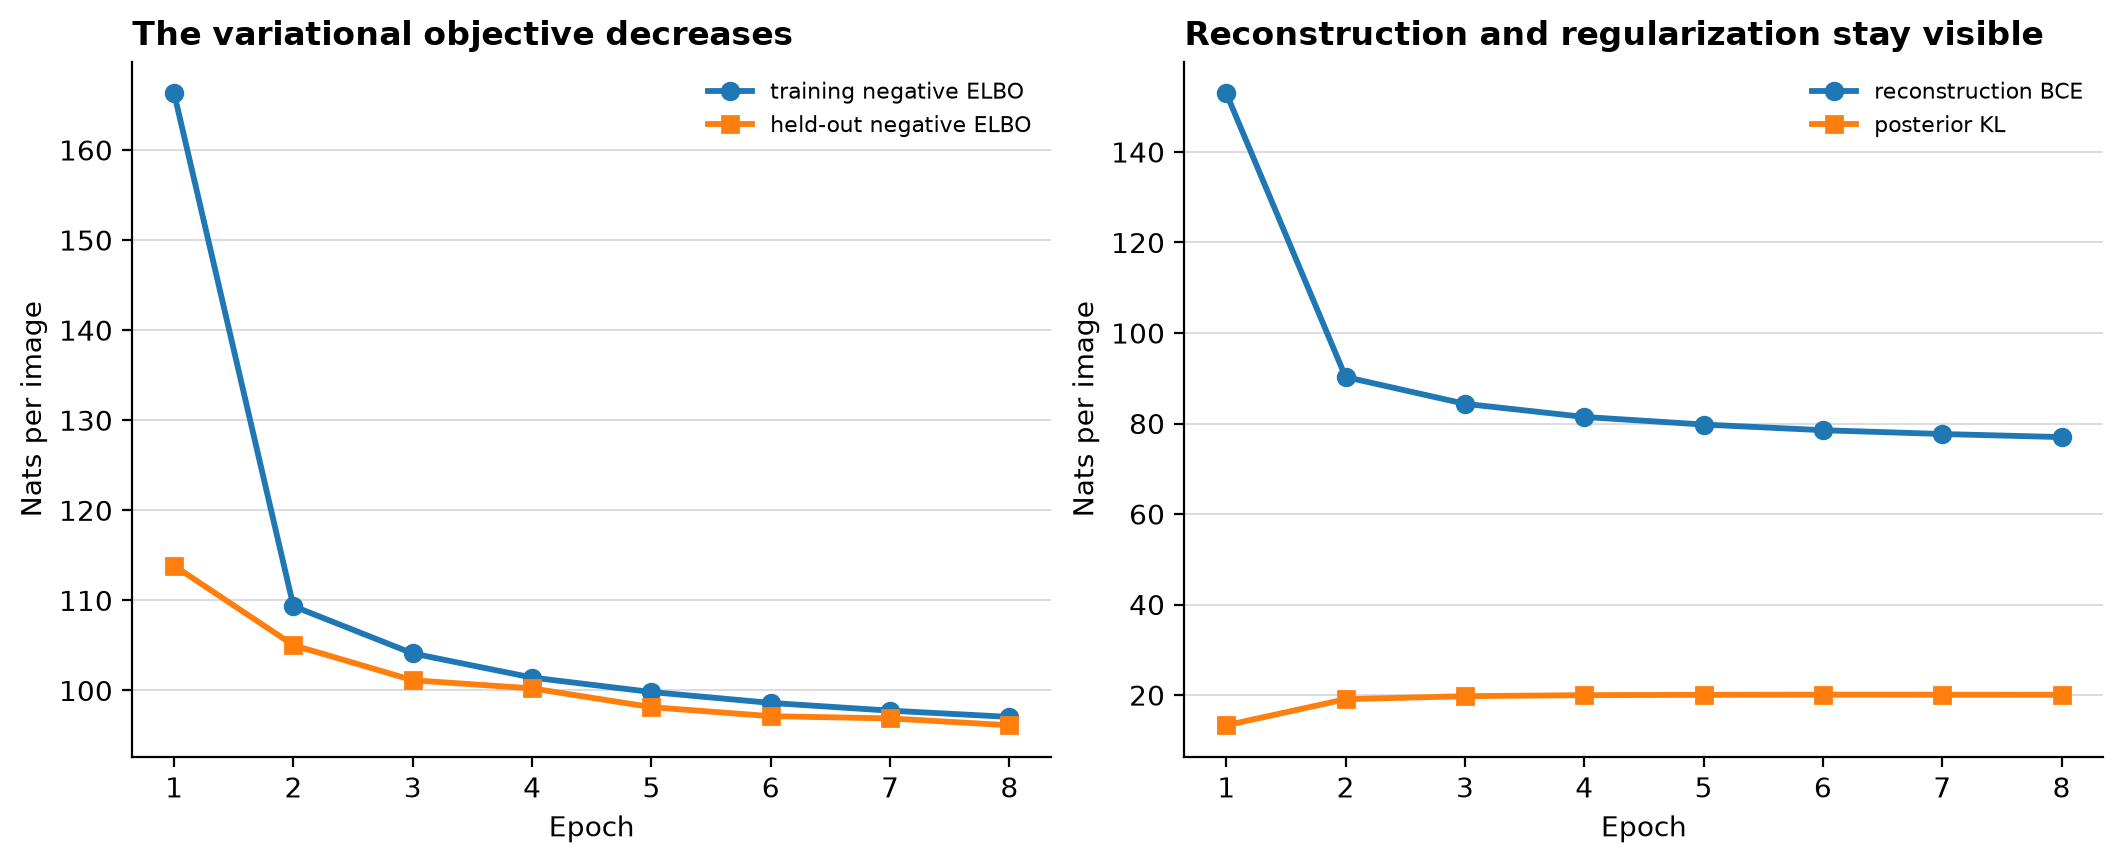
\includegraphics[width=0.88\linewidth]{mnist_28_vae_training_curve.png}
\caption{Training and held-out negative ELBO, with reconstruction BCE and
posterior KL shown separately. A nonzero KL shows that this run did not collapse
to the standard prior, although it does not prove that every latent coordinate
is useful.}
\end{figure}

After eight epochs, held-out negative ELBO was $96.14$ nats per image:
$76.70$ reconstruction BCE plus $19.44$ KL. The VAE probe scored $94.7\%$ on
held-out real digits and agreed with requested labels on $87.5\%$ of 80 generated
images. Its generated median nearest-training distance was $1.845$, compared
with $1.781$ for held-out data in the same 14-by-14 feature space. These results
support objective learning, useful one-pass conditional generation, and imperfect
control. They are not human recognizability, FID, or a privacy guarantee.


\section*{8. Empirical results and what they support}

\begin{figure}[H]
\centering
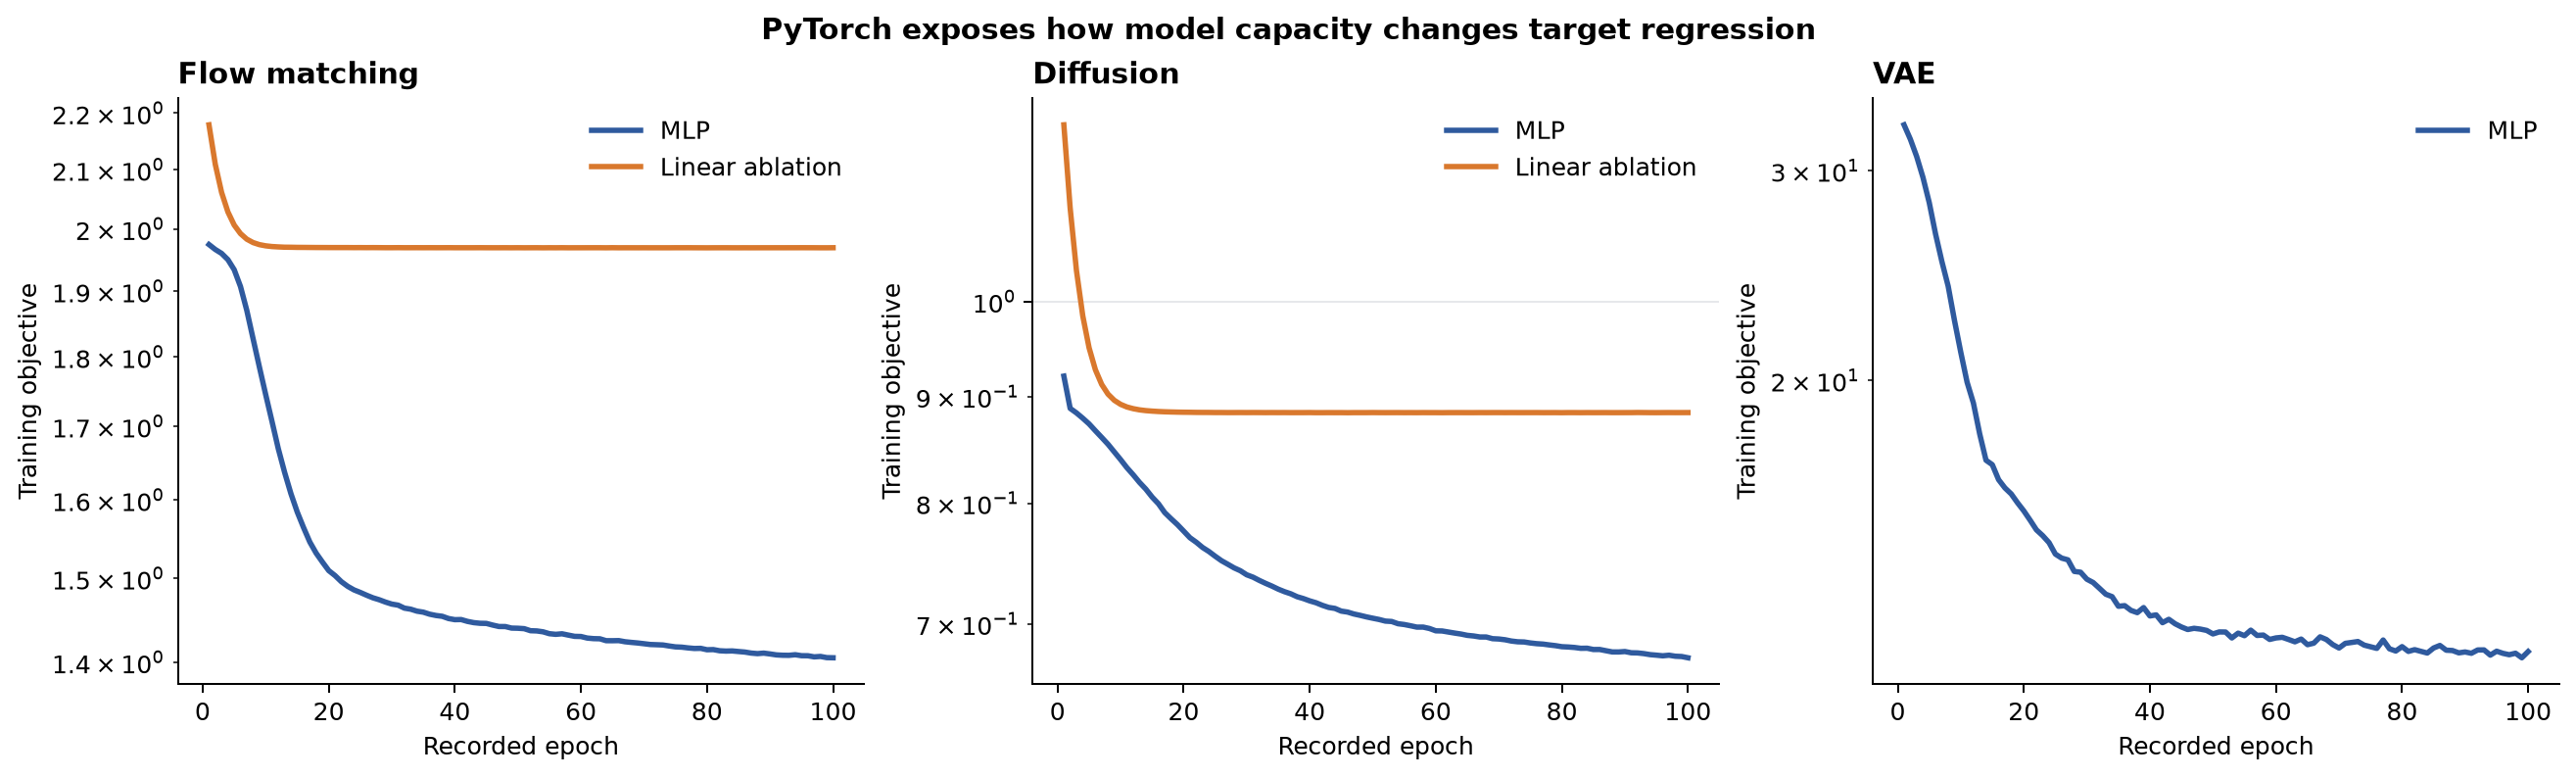
\includegraphics[width=0.96\linewidth]{learning_curves.png}
\caption{Optimization diagnostics. Flow/diffusion panels report regression MSE;
the VAE panel reports reconstruction cost plus KL. Held-out objectives are
reported separately and are not sample-quality metrics.}
\end{figure}

\begin{table}[H]
\centering
\scriptsize
\begin{tabular}{llrrrrrrr}
\toprule
Family & Impl. & Fr\'echet & MMD$^2$ & Prec. & Recall & Entropy & Classes & NN dist. \\
\midrule
Diffusion & linear ablation & 0.095 & 0.0018 & 0.455 & 0.806 & 0.984 & 10.0 & 1.471 \\
Diffusion & mlp & 0.116 & 0.0023 & 0.733 & 0.945 & 0.994 & 10.0 & 1.103 \\
Flow matching & linear ablation & 0.095 & 0.0018 & 0.440 & 0.814 & 0.987 & 10.0 & 1.487 \\
Flow matching & mlp & 0.133 & 0.0021 & 0.761 & 0.926 & 0.993 & 10.0 & 1.056 \\
Gaussian mixture & classical baseline & 0.090 & 0.0014 & 0.823 & 0.876 & 0.996 & 10.0 & 0.954 \\
VAE & mlp & 0.262 & 0.0046 & 0.644 & 0.849 & 0.978 & 10.0 & 1.247 \\
\bottomrule
\end{tabular}
\caption{Means over 8 paired sampling seeds,
500 samples per seed. Metrics are complementary,
not a composite leaderboard.}
\end{table}

\begin{figure}[H]
\centering
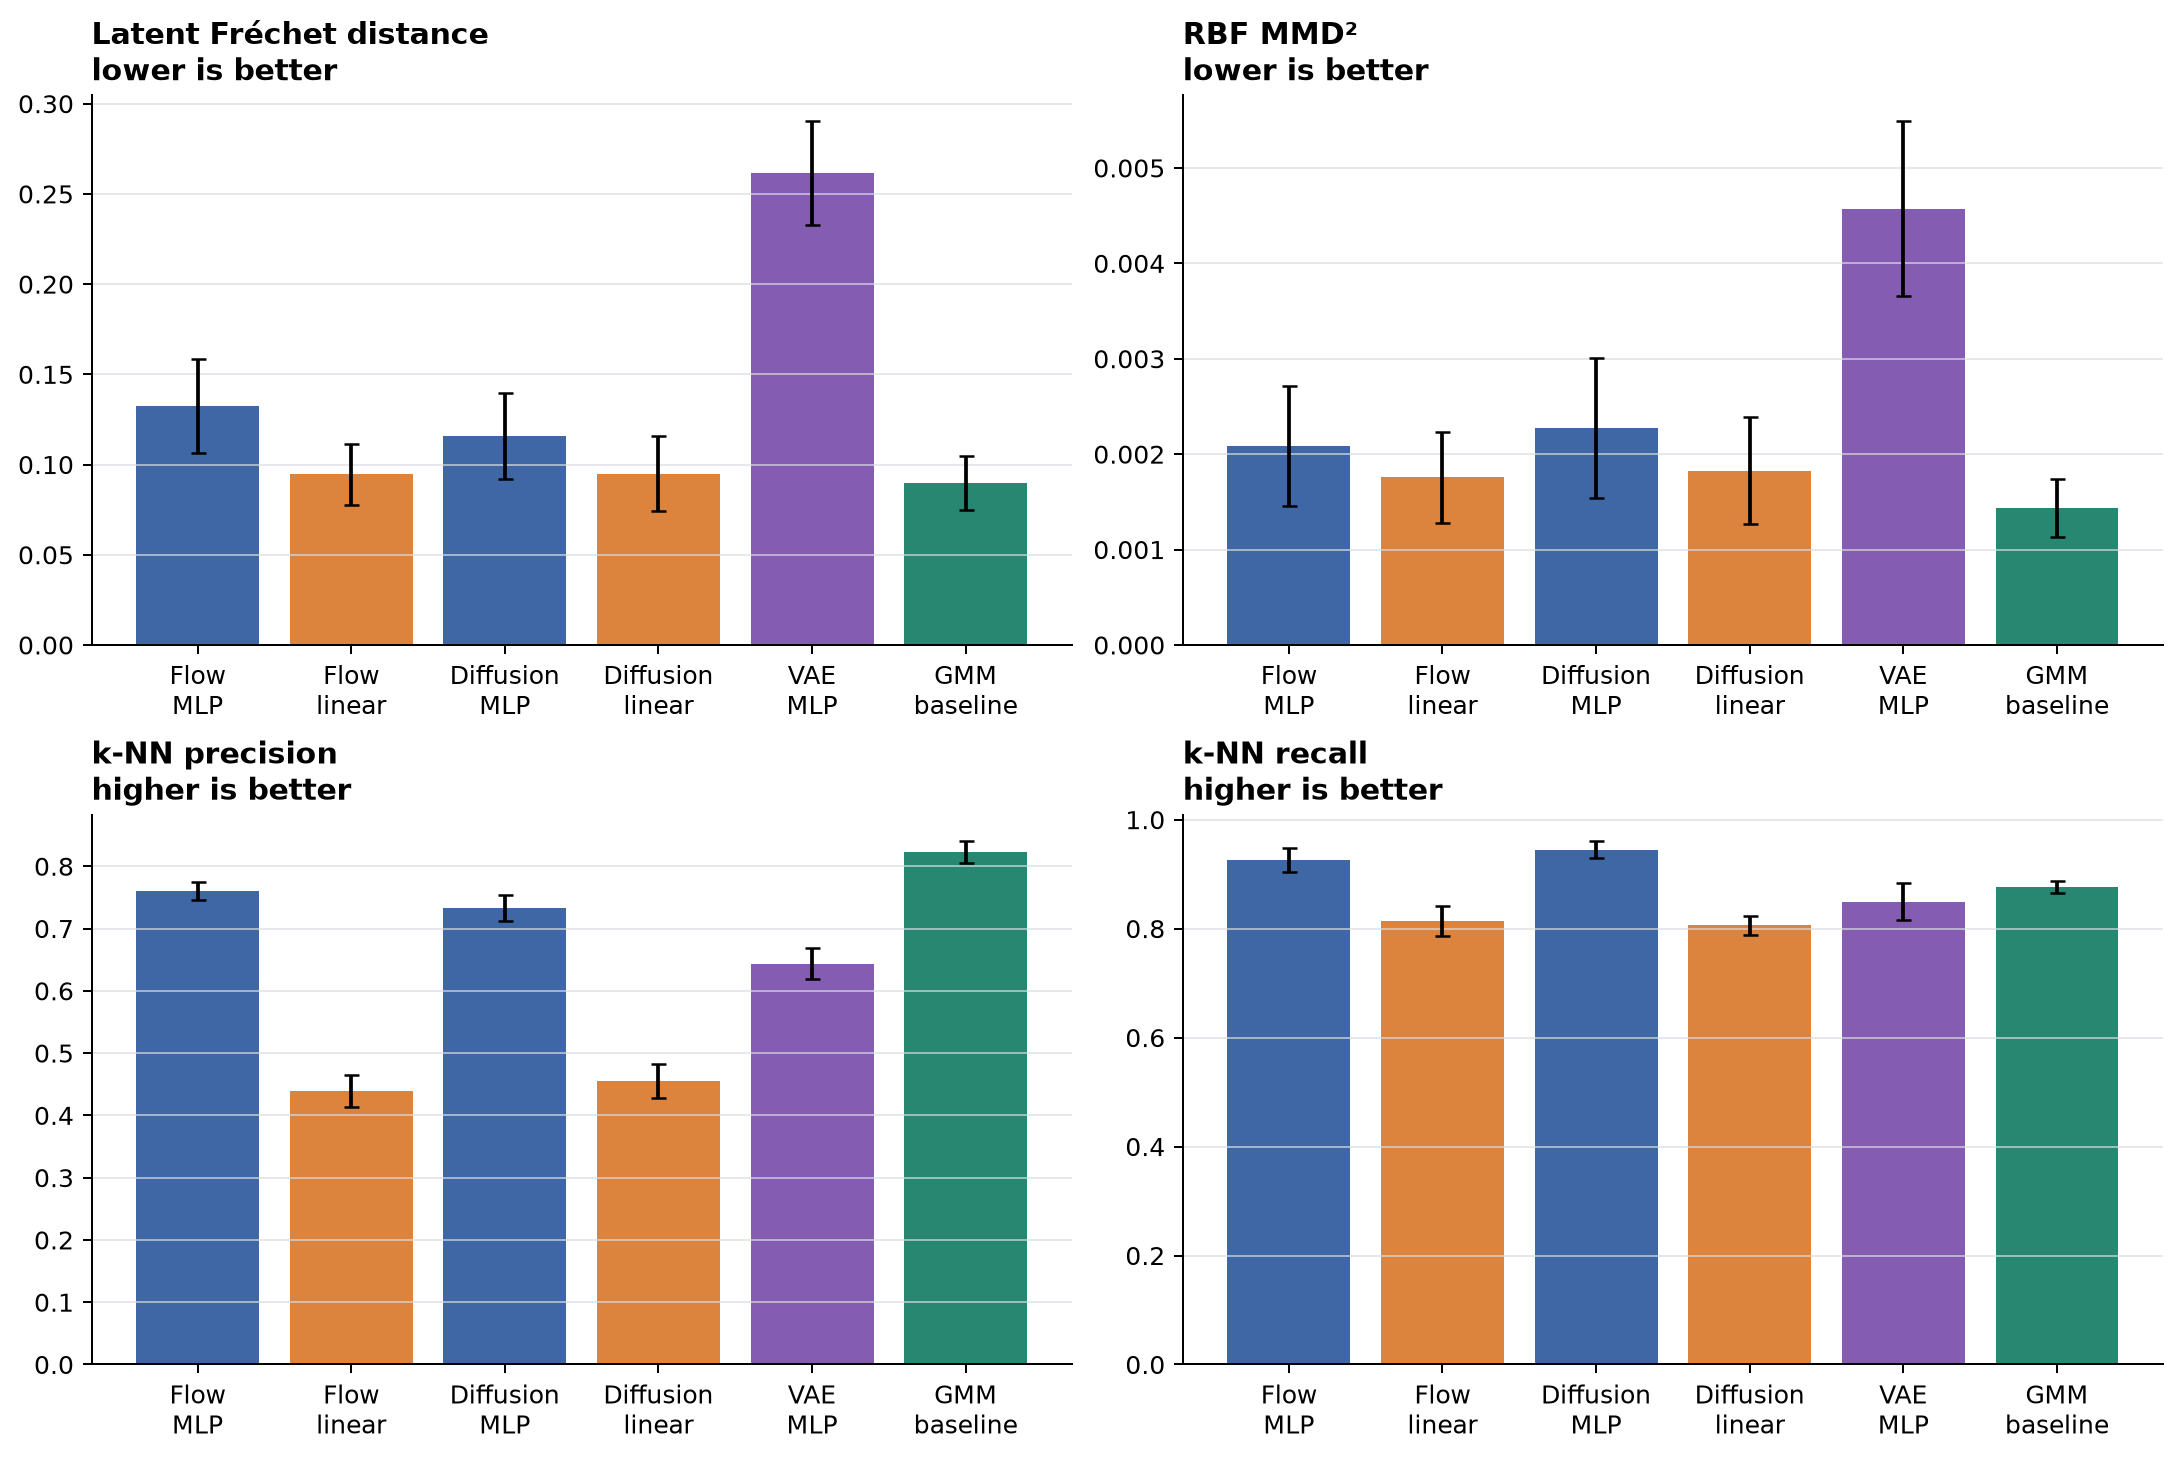
\includegraphics[width=0.92\linewidth]{distribution_metrics.png}
\caption{A single metric can reward one failure mode and hide another. Bars are
means and error bars are standard deviations across sample-generation seeds.}
\end{figure}

The precision/recall split follows the principle that fidelity and coverage are
separate axes \cite{sajjadi2018precision}. MMD detects broader distributional
differences; class entropy and class coverage diagnose mode omission through a
fixed digit probe; median nearest-training distance is a basic copying diagnostic.
None replaces conditional, human, subgroup, or application-specific evaluation.

\begin{table}[H]
\centering
\small
\begin{tabular}{llrrr}
\toprule
Family & Metric & MLP mean & Linear mean & MLP--linear [95\% interval] \\
\midrule
Flow matching & frechet\_latent & 0.1326 & 0.0946 & +0.0380 [+0.0271, +0.0499] \\
Flow matching & mmd\_rbf & 0.0021 & 0.0018 & +0.0003 [+0.0002, +0.0004] \\
Flow matching & precision\_knn & 0.7608 & 0.4395 & +0.3213 [+0.3043, +0.3390] \\
Flow matching & recall\_knn & 0.9264 & 0.8142 & +0.1122 [+0.0990, +0.1250] \\
Diffusion & frechet\_latent & 0.1158 & 0.0950 & +0.0208 [+0.0129, +0.0283] \\
Diffusion & mmd\_rbf & 0.0023 & 0.0018 & +0.0004 [+0.0003, +0.0006] \\
Diffusion & precision\_knn & 0.7330 & 0.4547 & +0.2782 [+0.2615, +0.2945] \\
Diffusion & recall\_knn & 0.9451 & 0.8063 & +0.1389 [+0.1281, +0.1521] \\
\bottomrule
\end{tabular}
\caption{Paired bootstrap across generation seeds. Intervals quantify Monte
Carlo sampling variation conditional on one fitted model; they exclude retraining
uncertainty and must not be read as a population confidence interval.}
\end{table}

\begin{figure}[H]
\centering
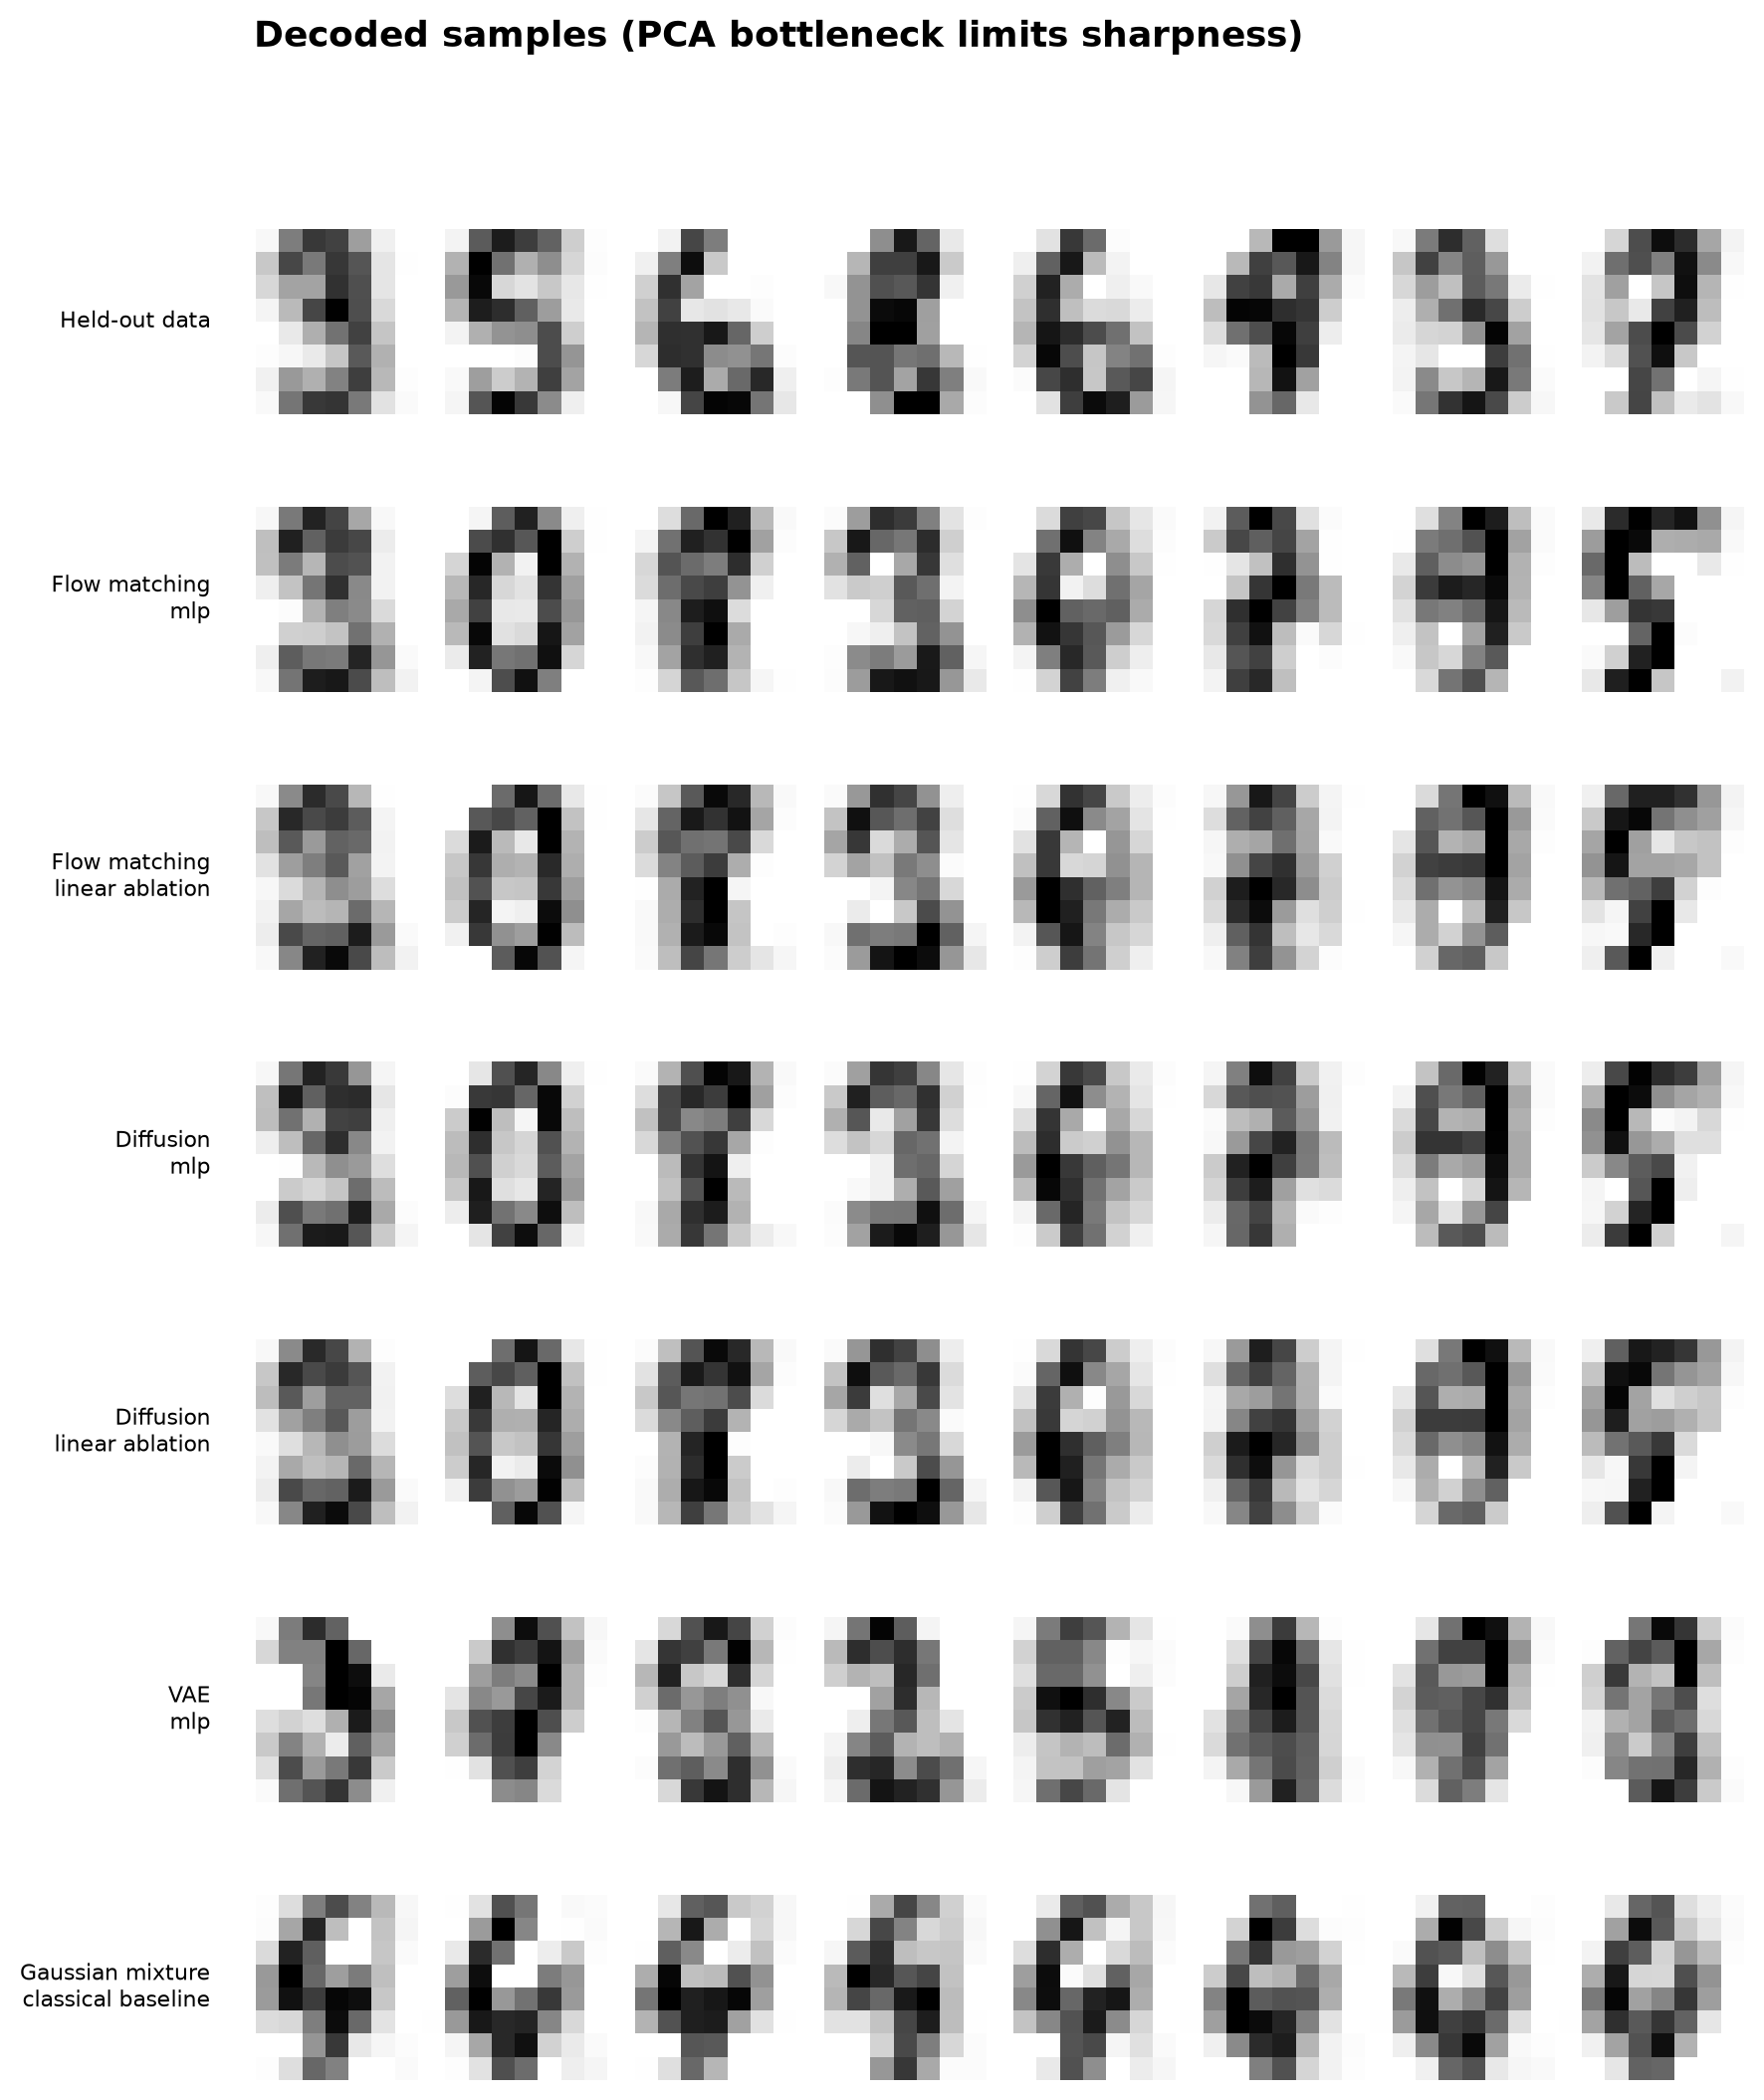
\includegraphics[width=0.95\linewidth]{decoded_sample_grid.png}
\caption{Decoded examples support visual debugging, not quantitative claims.
Every row uses the same training-fitted PCA inverse and display scale.}
\end{figure}

\begin{figure}[H]
\centering
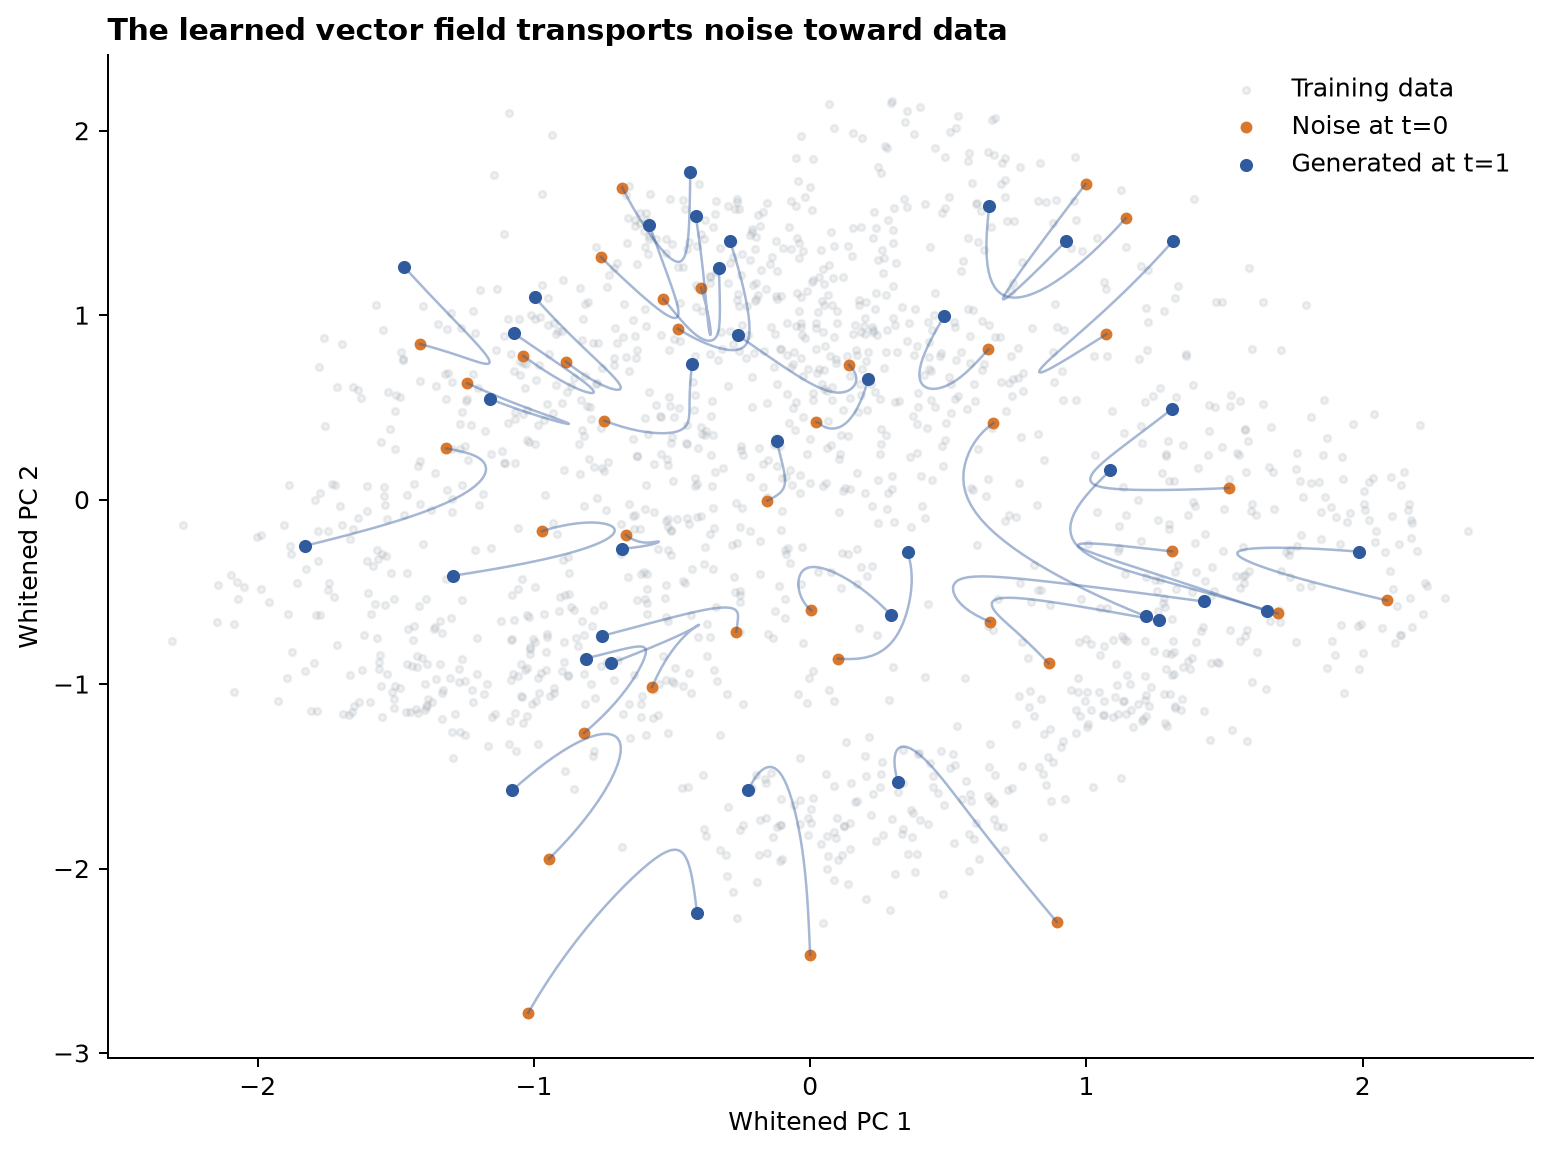
\includegraphics[width=0.86\linewidth]{flow_trajectories.png}
\caption{First two latent coordinates of PyTorch MLP flow-matching trajectories.
The full eight-dimensional integration is used for metrics.}
\end{figure}

\section*{9. Numerical cost and sampler sensitivity}

\begin{table}[H]
\centering
\small
\begin{tabular}{lrrrrr}
\toprule
Family & Steps & Network evals. & Batch sec. & Fr\'echet & MMD$^2$ \\
\midrule
Diffusion & 5 & 5 & 0.005 & 0.148 & 0.0022 \\
Diffusion & 10 & 10 & 0.008 & 0.132 & 0.0018 \\
Diffusion & 20 & 20 & 0.014 & 0.127 & 0.0016 \\
Diffusion & 50 & 50 & 0.034 & 0.125 & 0.0016 \\
Flow matching & 5 & 20 & 0.017 & 0.158 & 0.0017 \\
Flow matching & 10 & 40 & 0.030 & 0.158 & 0.0017 \\
Flow matching & 20 & 80 & 0.048 & 0.158 & 0.0017 \\
Flow matching & 30 & 120 & 0.071 & 0.158 & 0.0017 \\
VAE & 1 & 1 & 0.001 & 0.312 & 0.0058 \\
\bottomrule
\end{tabular}
\caption{PyTorch samplers on one fixed seed. RK4 uses four vector-field
evaluations per step; deterministic diffusion uses one noise prediction per
step; the VAE uses one decoder evaluation.}
\end{table}

\begin{figure}[H]
\centering
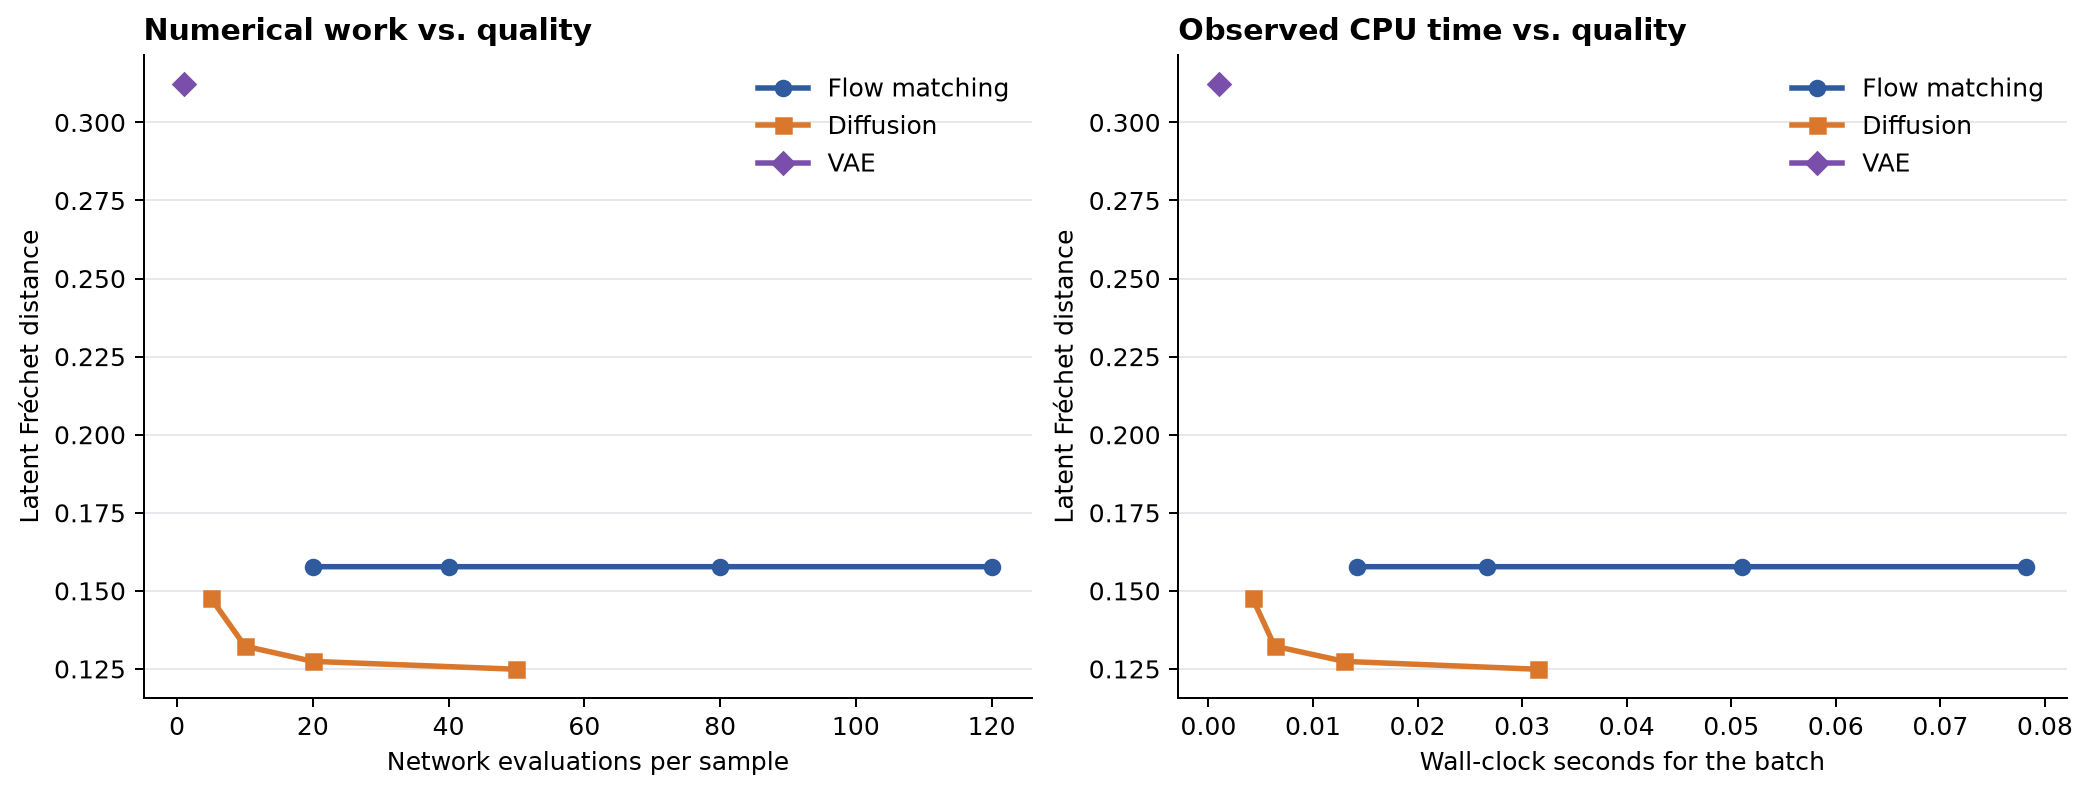
\includegraphics[width=0.88\linewidth]{sampling_tradeoff.png}
\caption{Step count is both a numerical-analysis parameter and a deployment-cost
parameter. A fair comparison reports network evaluations and quality together.}
\end{figure}

\section*{10. Assessment plan and companion homework}

The student-facing assignment uses Fashion-MNIST, not digits. Students implement
or extend VAE, flow, and diffusion objectives, verify analytic identities, define
PyTorch \code{nn.Module} models, train them with autograd and Adam, compare a
flow capacity ablation, contrast one-pass and iterative samplers, and write a
short model card. The
assignment is scoped so a CPU-only reduced subset is valid; an optional extension
may replace the PCA/MLP backbone with a convolutional PyTorch architecture without
changing the mathematical tests.

Suggested grading weights are: derivations 20\%, implementation correctness and
tests 25\%, controlled experiment 25\%, evaluation/uncertainty 20\%, and
reproducibility/communication 10\%. Solutions specify exact derivations where
available and explicit criteria for open-ended design judgments.

\section*{11. Limitations and capstone extensions}

\begin{itemize}
\item \textbf{Capacity.} PCA plus small MLPs cannot represent image detail that
modern convolutional or transformer backbones capture.
\item \textbf{Conditioning scope.} The controlled 8-by-8 benchmark is
unconditional; the 28-by-28 MNIST demonstration is label-conditional. Neither
tests free-form conditioning or classifier-free guidance.
\item \textbf{One training seed.} Paired generation seeds quantify sampler
variation, not optimization variability. A research claim requires repeated fits.
\item \textbf{Metric validity.} The benchmark lacks perceptual features, human
evaluation, calibrated privacy attacks, subgroup analysis, and downstream utility.
\item \textbf{Path and schedule.} Independent flow coupling and a linear beta
schedule are transparent baselines, not universally optimal choices.
\item \textbf{Variational family.} Diagonal Gaussian posteriors, fixed decoder
likelihoods, and $\beta=1$ are transparent VAE choices, not universally optimal;
the two-moons prior mismatch visibly smooths between modes.
\item \textbf{Density.} The benchmark does not estimate CNF likelihood through
the divergence integral; the affine-flow unit separately validates exact density.
\end{itemize}

Strong capstone extensions include minibatch OT flow matching, conditional
generation, probability-flow ODE comparison, latent diffusion, score calibration,
Schr\"odinger bridges, discrete/categorical flows, likelihood estimation with
Hutchinson traces, and a domain-specific evaluation protocol. LLMs can be added
later as a separate autoregressive sequence-modeling module.

\section*{12. Reproducibility map}

The build has one numerical source of truth and stable topic-scoped outputs:
\begin{itemize}
\item experiment: \path{experiments/generative/run_benchmark.py};
\item visual experiments: \path{experiments/generative/run_visual_examples.py};
\item reusable code: \path{src/math550/topics/generative};
\item mathematical tests: \path{tests/generative};
\item tables and figures: \path{output/generative/analysis} and
\path{output/generative/figures}; and
\item classroom artifacts: \path{slides/generative} and
\path{homework/generative}.
\end{itemize}
The JSON run configuration records the split, PCA, target paths, schedules,
architecture, PyTorch version/device, seeds, sample counts, and metric scope.
The separate \path{visual_examples.json} records MNIST checksums, the exact
two-moons Code 1 settings, VAE likelihood/posterior choices, component-wise
training curves, sampler settings, probes, and caveats.


\clearpage
\section*{Teaching companion: derivations, checks, and discussion prompts}

The preceding sections are the evidence record. This companion turns that
record into a sequence of derivations and classroom decisions. Each subsection
has three parts: a mathematical object, a check that can fail, and a question
that forces students to interpret rather than merely execute code.

\subsection*{A. What a generator is actually learning}

Let $P_{\rm data}$ be the unknown population distribution and let
$x_1,\ldots,x_n$ be the observed sample. A generator defines a model
distribution $P_\theta$ from which new observations can be drawn. Three claims
must be kept separate:

\begin{enumerate}
\item \emph{fit}: $P_\theta$ matches aspects of the empirical distribution;
\item \emph{generalization}: those aspects also match unseen population draws;
\item \emph{utility}: generated observations are useful for a declared task.
\end{enumerate}

An exact likelihood can test the first two claims under a density model, but it
does not by itself establish perceptual fidelity or downstream utility. An
implicit generator may produce attractive samples while assigning no accessible
density. This is why the module treats likelihood, sample quality, coverage,
memorization, and compute as distinct axes.

\textbf{Check.} Ask whether every reported metric has a named reference set,
representation, sample count, and direction of improvement.

\textbf{Discuss.} Can two generators have identical likelihood and different
sample quality? Can they have identical sample quality and different coverage?

\subsection*{B. Autoregressive likelihood and latent-variable bounds}

The chain rule gives an exact factorization for any ordering:
\[
 p_\theta(x)=\prod_{j=1}^d p_\theta(x_j\mid x_{<j}),\qquad
 \log p_\theta(x)=\sum_{j=1}^d\log p_\theta(x_j\mid x_{<j}).
\]
Training can evaluate all observed conditionals in parallel when masking is
available, but ancestral sampling remains sequential in the chosen order. The
factorization is exact; the conditional model and its inductive biases are not.

For a latent-variable model, insert any distribution $q_\phi(z\mid x)$ and use
Jensen's inequality:
\begin{align*}
 \log p_\theta(x)
 &=\log\int q_\phi(z\mid x)
   \frac{p_\theta(x,z)}{q_\phi(z\mid x)}\,dz\\
 &\geq \E_{q_\phi(z\mid x)}[\log p_\theta(x\mid z)]
 -D_{\rm KL}\!\left(q_\phi(z\mid x)\Vert p(z)\right).
\end{align*}
The gap is $D_{\rm KL}(q_\phi(z\mid x)\Vert p_\theta(z\mid x))$. A tight
bound therefore requires an expressive decoder \emph{and} an adequate
approximate posterior. The reparameterization
$z=\mu_\phi(x)+\sigma_\phi(x)\odot\epsilon$ with
$\epsilon\sim\mathcal N(0,I)$ moves randomness outside the differentiable
network path.

\textbf{Check.} Verify that the KL term and reconstruction term use compatible
reductions. A sum over pixels and a mean over latent dimensions silently changes
their relative weight.

\textbf{Discuss.} Why can a powerful decoder ignore $z$? Which diagnostic would
distinguish posterior collapse from merely noisy latent coordinates?

\subsection*{B.1 The executable VAE contract}

The vector VAE uses a fixed-variance Gaussian decoder, so its per-example
negative ELBO (up to a parameter-independent constant) is
\[
 \frac{1}{2\sigma_x^2}\lVert x-\mu_\theta(z)\rVert_2^2
 +\frac12\sum_j\left[
 \mu_{\phi,j}(x)^2+\exp(\log\sigma_{\phi,j}^2(x))
 -1-\log\sigma_{\phi,j}^2(x)\right].
\]
The MNIST VAE replaces the Gaussian reconstruction cost with a 784-pixel
Bernoulli binary cross-entropy and conditions both encoder and decoder on the
digit label. Both are ordinary \code{torch.nn.Module} models; the course logic
keeps the posterior parameterization, reparameterized noise, reductions,
component-wise diagnostics, and prior sampler explicit.

\textbf{Check.} Assert a zero KL for $\mu=0,\log\sigma^2=0$, finite gradients for
both posterior heads, native output shape, and separate train/held-out curves for
reconstruction, KL, and total objective.

\textbf{Discuss.} Why can low reconstruction error coexist with poor prior
samples on a thin multimodal target?

\subsection*{C. Adversarial objectives and density ratios}

For fixed generator $G$, maximizing the original GAN value pointwise gives
\[
 D^*(x)=\frac{p_{\rm data}(x)}{p_{\rm data}(x)+p_G(x)}.
\]
Substitution yields a Jensen--Shannon divergence objective up to an additive
constant. This result assumes an optimal discriminator and overlapping support;
neither is guaranteed during finite alternating optimization. The common
non-saturating generator loss $-\E_z\log D(G(z))$ improves gradients but changes
the game followed by the actual iterates.

\textbf{Check.} Plot discriminator and generator losses together with held-out
coverage. A stable scalar loss is not evidence that modes are retained.

\textbf{Discuss.} What failure would be missed if a human evaluator sees only a
curated grid of high-quality samples?

\subsection*{D. Discrete flows and triangular Jacobians}

Suppose an affine coupling layer partitions $x=(x_a,x_b)$ and defines
\[
 y_a=x_a,\qquad y_b=x_b\odot\exp s_\theta(x_a)+t_\theta(x_a).
\]
The inverse is explicit:
\[
 x_a=y_a,\qquad
 x_b=(y_b-t_\theta(y_a))\odot\exp[-s_\theta(y_a)].
\]
The Jacobian is triangular, so
$\log|\det J|=\sum_j s_{\theta,j}(x_a)$. The neural networks $s_\theta$ and
$t_\theta$ are ordinary PyTorch modules; the architecture, not a hand-derived
neural optimizer, makes the determinant tractable.

\textbf{Check.} Numerically verify round-trip error and cancellation of forward
and inverse log determinants on random inputs before fitting any data.

\textbf{Discuss.} Why does exact invertibility restrict dimension-changing
operations? How do multiscale flows work around this constraint?

\subsection*{E. Continuous transport and the flow-matching identity}

Let $\phi_t$ solve $d\phi_t(x)/dt=u_t(\phi_t(x))$. Conservation of mass implies
\[
 \partial_t p_t(x)+\nabla\cdot[p_t(x)u_t(x)]=0.
\]
Along a trajectory this becomes
\[
 \frac{d}{dt}\log p_t(X_t)=-\nabla\cdot u_t(X_t).
\]
Continuous normalizing flows can integrate both state and density, but evaluating
the divergence can be expensive in high dimension.

Conditional flow matching avoids solving an ODE inside each training update.
Let $Z$ index a tractable conditional path with density $p_t(x\mid Z)$ and field
$u_t(x\mid Z)$. Define
\[
 p_t(x)=\int p_t(x\mid z)p(z)\,dz,
 \quad
 u_t(x)=\frac{\int u_t(x\mid z)p_t(x\mid z)p(z)\,dz}{p_t(x)}.
\]
Conditioning on $X_t=x$ shows that
$u_t(x)=\E[u_t(X_t\mid Z)\mid X_t=x]$. Squared-error regression therefore has
the same population minimizer whether it targets the unavailable marginal field
or sampled conditional fields. The conditional target is not an approximation
to a known marginal target; it is a stochastic regression target whose
conditional mean is the desired field.

For the classroom interpolation,
\[
 X_t=[1-(1-\sigma_{\min})t]X_0+tX_1,
 \qquad
 \dot X_t=X_1-(1-\sigma_{\min})X_0.
\]
The target is analytic. The learned model receives $[t,X_t]$ and predicts a
vector with the same dimension as $X_t$.

\textbf{Check.} Use finite differences to verify
$(X_{t+h}-X_t)/h\approx\dot X_t$, and test that an affine field reproduces a
known Gaussian transport before interpreting learned samples.

\textbf{Discuss.} Independent endpoint coupling is cheap. Why can an
optimal-transport coupling reduce path curvature, and what new estimation
dependence does minibatch coupling introduce?

\subsection*{E.1 The three-example evidence ladder}

The module deliberately assigns different jobs to three demonstrations. The
two-moons experiment reproduces the guide's page-7 Code 1 settings, makes
particle transport visible, and exposes VAE prior mismatch. Original 28-by-28
MNIST compares recognizable label-controlled flow and one-pass VAE generation.
The 8-by-8 PCA benchmark sacrifices sharpness so VAE, flow, diffusion, baselines,
seeds, metrics, and numerical budgets can be compared cheaply.
No one example is asked to prove mechanism, realism, and broad performance at
the same time.

\textbf{Check.} For every classroom claim, name which example supplies the
evidence and whether the evidence is visual, mathematical, or quantitative.

\textbf{Discuss.} Why would replacing the controlled PCA benchmark with only a
curated MNIST grid weaken the module, even though the grid is more visually
compelling?

\subsection*{F. ODE solvers are part of the model contract}

Euler's method uses
$x_{k+1}=x_k+h v_\theta(t_k,x_k)$ and has global error $O(h)$. Classical RK4
combines four field evaluations per step and has global error $O(h^4)$ under
regularity conditions. Consequently, ``30 steps'' is not a fair compute label
unless the solver and its number of network evaluations are also stated.

Three errors can be separated experimentally:
\begin{enumerate}
\item \emph{regression error}: the learned field misses its conditional target;
\item \emph{path error}: the chosen probability path is difficult or undesirable;
\item \emph{integration error}: a finite-step solver misses the learned flow.
\end{enumerate}
Holding two components fixed while varying the third turns vague sample-quality
complaints into a diagnostic experiment.

\textbf{Check.} Halve the step size and compare endpoints. If samples change
substantially while training loss is fixed, numerical error is material.

\subsection*{G. Diffusion objectives from the forward marginal}

Let $\alpha_t=1-\beta_t$ and
$\bar\alpha_t=\prod_{s=1}^t\alpha_s$. Repeated Gaussian transitions give
\[
 x_t=\sqrt{\bar\alpha_t}x_0+\sqrt{1-\bar\alpha_t}\epsilon,
 \qquad \epsilon\sim\mathcal N(0,I).
\]
This closed form permits uniform sampling of time indices during training. A
noise-prediction network minimizes
\[
 \E\left\|\epsilon-\epsilon_\theta(x_t,t)\right\|_2^2.
\]
Equivalent parameterizations predict $x_0$, the score, or a velocity-like
combination, but their weighting and numerical behavior differ across signal-to-
noise ratios. The score identity is
\[
 \nabla_{x_t}\log q(x_t\mid x_0)
 =-\frac{\epsilon}{\sqrt{1-\bar\alpha_t}}.
\]

For deterministic DDIM-style sampling, estimate
\[
 \hat x_0=\frac{x_t-\sqrt{1-\bar\alpha_t}\,epsilon_\theta(x_t,t)}
 {\sqrt{\bar\alpha_t}}
\]
and combine $\hat x_0$ with the predicted noise at the next selected time. Skipping
times changes the numerical path; it does not retrain the network.

\textbf{Check.} Substitute the true noise into the reconstruction formula and
verify recovery of $x_0$ to floating-point tolerance.

\textbf{Discuss.} Why do very low signal-to-noise times amplify error in an
$x_0$ reconstruction? How might loss weighting respond?

\subsection*{H. Reverse SDE and probability-flow ODE}

For a forward SDE
\[
 dX=f(X,t)\,dt+g(t)\,dW_t,
\]
the reverse-time dynamics depend on the score $s_t(x)=\nabla_x\log p_t(x)$:
\[
 dX=[f(X,t)-g(t)^2s_t(X)]\,dt+g(t)\,d\bar W_t,
\]
with time run backward. The probability-flow ODE
\[
 dX=[f(X,t)-\tfrac12g(t)^2s_t(X)]\,dt
\]
has the same marginal densities under the required regularity conditions. Same
marginals do not mean identical sample paths. Stochasticity, solver choice, and
conditioning can change individual outputs and compute.

\textbf{Check.} State whether a reported sampler is stochastic or deterministic,
which time grid it uses, and how many neural evaluations one sample requires.

\subsection*{I. PyTorch implementation and device discipline}

The module uses \code{torch.nn.Module}, standard linear/convolutional layers and
activations, \code{MSELoss}, binary cross-entropy, autograd, and PyTorch
optimizers.
The code does not reimplement neural layers or backpropagation. A command-line
device request can be \code{auto}, \code{cuda}, \code{mps}, or \code{cpu}.
The \code{auto} policy resolves CUDA first, then Apple Metal, then CPU; an
explicit unavailable accelerator raises an error. The fitted network, training
tensors, validation tensors, and prediction tensors share the resolved device,
which is recorded in the run metadata.

\begin{verbatim}
model = TorchVectorRegressor(
    hidden_sizes=(64, 64), model_kind="mlp", device="auto"
)
model.fit(train_features, train_targets,
          validation_features, validation_targets)
print(model.device_)
\end{verbatim}

Reproducibility includes more than a seed: report the PyTorch version, device,
data split, preprocessing fit scope, training-pair generator, optimizer, batch
size, epoch budget, and sampler grid. Accelerator kernels may still differ from
CPU arithmetic even under deterministic settings.

\textbf{Check.} Assert that every model parameter has the same device type as
the resolved device, and run a tiny CPU test in continuous integration.

\subsection*{J. Reading the public-data evidence}

The experiment uses 1,437 training images and 360 untouched test images. PCA is
fit on training rows only; its eight whitened coordinates retain 67.4\% of
training variance. This bottleneck makes the experiment inexpensive and exposes
metric mechanics, but it also places a hard ceiling on decoded detail.

The Gaussian mixture achieved the smallest mean latent Fr\'echet distance
(0.090). The flow-matching MLP achieved 0.133 and the matched linear ablation
0.095; the paired MLP-minus-linear difference was +0.038 with a 95\% interval
[+0.027,+0.050]. The MLP nevertheless gained about 0.321 in k-NN precision.
This apparent conflict is useful: Fr\'echet compares only Gaussian moments,
whereas local precision responds to sample neighborhoods. Neither number alone
declares a winner.

For diffusion, the MLP validation noise-prediction MSE (0.731) improved over the
linear ablation (0.895), but its mean latent Fr\'echet distance (0.116) remained
worse than the linear result (0.095). A better supervised objective can be
necessary without being sufficient for a better finite-step generator.

\textbf{Check.} Before interpreting any Fr\'echet number, name its feature space.
The reported quantity is not Inception FID.

\subsection*{K. A reusable evaluation protocol}

\begin{enumerate}
\item Freeze the train/test split and fit every representation on training data.
\item Use held-out real data as the distributional reference.
\item Run paired generation seeds so model differences share random conditions.
\item Report at least one global discrepancy, one local precision/coverage pair,
one memorization diagnostic, decoded samples, and compute.
\item Add confidence intervals for a declared comparison, not only standard
deviations for each model in isolation.
\item Inspect failures and disclose the representation, sample count, fitting
seeds, and sampler configuration.
\end{enumerate}

Nearest-training distance is a screen, not a privacy guarantee. A serious release
decision needs stronger membership-inference or exposure tests, subgroup analysis,
rights review, and a response plan for memorized or harmful samples.

\subsection*{L. Nine-unit instructor plan}

\begin{center}
\small
\begin{tabularx}{\linewidth}{p{0.07\linewidth}p{0.23\linewidth}X}
\toprule
Unit & Board derivation & Studio or exit evidence \\
\midrule
1 & Distribution claims and metric axes & Critique a one-metric model card \\
2 & ELBO and reparameterization & Diagnose a reduction or collapse bug \\
3 & GAN density ratio & Design a mode-coverage audit \\
4 & Coupling inverse and log determinant & Pass round-trip and log-det tests \\
5 & Continuity equation and CNF density & Separate state and density ODEs \\
6 & Conditional FM identity & Verify target velocity and solver convergence \\
7 & Diffusion forward marginal & Pass oracle reconstruction test \\
8 & Reverse SDE and probability-flow ODE & Compare stochastic and deterministic costs \\
9 & Paired benchmark interpretation & Defend a capstone model and failure policy \\
\bottomrule
\end{tabularx}
\end{center}

Each unit can be taught as 35 minutes of derivation, 15 minutes of code or
diagnostics, and 10 minutes of critique. Across a three-hour week, the remaining
time supports a longer evidence lab and a short break.

\subsection*{M. Glossary}

\begin{description}
\item[Coverage] Whether the generator represents the diversity or modes of the
target distribution.
\item[Explicit density] A model for which normalized $p_\theta(x)$ or a tractable
equivalent can be evaluated.
\item[Implicit model] A model that can sample but does not expose a tractable
normalized density.
\item[Probability path] A family $(p_t)_{t\in[0,1]}$ connecting a base and target
distribution.
\item[Pushforward] The distribution obtained by applying a map to a random
variable, written $f_\#P$.
\item[Score] The gradient $\nabla_x\log p_t(x)$.
\item[Vector field] A function assigning an instantaneous velocity to every time
and state.
\item[Network evaluation] One forward call to the learned neural field or
denoiser; a more comparable sampler-cost unit than raw step count.
\end{description}

\clearpage
\begin{thebibliography}{99}
\bibitem{lipman2024guide} Y. Lipman et al. \emph{Flow Matching Guide and Code}.
arXiv:2412.06264, 2024. \url{https://arxiv.org/abs/2412.06264}.
\bibitem{lipman2023flow} Y. Lipman et al. \emph{Flow Matching for Generative
Modeling}. ICLR, 2023. \url{https://arxiv.org/abs/2210.02747}.
\bibitem{chen2018neural} R. T. Q. Chen et al. \emph{Neural Ordinary
Differential Equations}. NeurIPS, 2018.
\url{https://proceedings.neurips.cc/paper/7892-neural-ordinary-differential-equations}.
\bibitem{dinh2017realnvp} L. Dinh, J. Sohl-Dickstein, and S. Bengio.
\emph{Density Estimation Using Real NVP}. ICLR, 2017.
\url{https://arxiv.org/abs/1605.08803}.
\bibitem{ho2020ddpm} J. Ho, A. Jain, and P. Abbeel. \emph{Denoising Diffusion
Probabilistic Models}. NeurIPS, 2020.
\url{https://proceedings.neurips.cc/paper/2020/hash/4c5bcfec8584af0d967f1ab10179ca4b-Abstract.html}.
\bibitem{song2021sde} Y. Song et al. \emph{Score-Based Generative Modeling
through Stochastic Differential Equations}. ICLR, 2021.
\url{https://openreview.net/forum?id=PxTIG12RRHS}.
\bibitem{song2021ddim} J. Song, C. Meng, and S. Ermon. \emph{Denoising Diffusion
Implicit Models}. ICLR, 2021. \url{https://arxiv.org/abs/2010.02502}.
\bibitem{salimans2022distill} T. Salimans and J. Ho. \emph{Progressive
Distillation for Fast Sampling of Diffusion Models}. ICLR, 2022.
\url{https://arxiv.org/abs/2202.00512}.
\bibitem{kingma2014vae} D. P. Kingma and M. Welling. \emph{Auto-Encoding
Variational Bayes}. ICLR, 2014. \url{https://arxiv.org/abs/1312.6114}.
\bibitem{goodfellow2014gan} I. Goodfellow et al. \emph{Generative Adversarial
Nets}. NeurIPS, 2014.
\url{https://papers.nips.cc/paper/5423-generative-adversarial-nets}.
\bibitem{oord2016pixel} A. van den Oord, N. Kalchbrenner, and K. Kavukcuoglu.
\emph{Pixel Recurrent Neural Networks}. ICML, 2016.
\url{https://proceedings.mlr.press/v48/oord16.html}.
\bibitem{sajjadi2018precision} M. S. M. Sajjadi et al. \emph{Assessing
Generative Models via Precision and Recall}. NeurIPS, 2018.
\url{https://proceedings.neurips.cc/paper/2018/hash/f7696a9b362ac5a51c3dc8f098b73923-Abstract.html}.
\bibitem{uciDigits} E. Alpaydin and C. Kaynak. \emph{Optical Recognition of
Handwritten Digits} [Dataset]. UCI Machine Learning Repository, 1998.
\url{https://doi.org/10.24432/C50P49}.
\bibitem{mnistOriginal} Y. LeCun, C. Cortes, and C. J. C. Burges.
\emph{The MNIST Database of Handwritten Digits} [Dataset].
\url{https://yann.lecun.org/exdb/mnist/}.
\bibitem{pytorchDocs} PyTorch Contributors. \emph{PyTorch Documentation}.
\url{https://docs.pytorch.org/docs/stable/}.
\end{thebibliography}

\end{document}
